\documentclass[a4paper,11pt]{article}
%
%--------------------   start of the 'preamble'
%
\usepackage{graphicx,amssymb,amstext,amsmath}
\usepackage[usenames]{color}
\usepackage{bm}
\usepackage {hyperref}
\usepackage{caption}
\usepackage{xcolor}
\usepackage[many]{tcolorbox}
\usepackage{verbatim}
\usepackage[utf8]{inputenc}
\usepackage[english]{babel}

%Import the natbib package and sets a bibliography  and citation styles
%\usepackage{natbib}
%\bibliographystyle{ksfh_nat}

\captionsetup[figure]{labelfont=bf,font={small, sf, it}}
\newcommand\etc{\textsl{etc}}
\newcommand\eg{\textsl{eg.}\ }
\newcommand\etal{\textsl{et al.}}
\newcommand\Quote[1]{\lq\textsl{#1}\rq}

\newcommand{\ket}[1]{| #1 \rangle}
\newcommand{\bra}[1]{\langle #1 |}
\newcommand{\braket}[2]{\langle #1 | #2 \rangle}
\newcommand{\proj}[1]{| #1\rangle\!\langle #1 |}
\newcommand{\id}{\mathbbm{1}}
\newcommand{\heff}{\tilde H}
\newcommand{\ueff}{\tilde U}
\newcommand{\nv}{N$-V$}
\newcommand{\nfourteen}{$^{14}$N}
\newcommand{\nfifteen}{$^{15}$N}
\newcommand{\cthirteen}{$^{13}$C}
\newcommand{\ctwelve}{$^{12}$C}
\newcommand {\Fig}[1] {Figure~\ref{#1}}
\newcommand{\dev}[2]{\frac{d #1}{d #2 }}
\newcommand{\secdev}[2]{\frac{d^2 #1}{d #2^2 }}
\newcommand{\pdev}[2]{\frac{\partial #1}{\partial #2 }}
\newcommand{\secpdev}[2]{\frac{\partial^2 #1}{\partial #2^2 }}
\newcommand{\beq}{\begin{equation}}
\newcommand{\eeq}{\end{equation}}
\newcommand{\baq}{\begin{eqnarray}}
\newcommand{\eaq}{\end{eqnarray}}
\newcommand{\diverg}[1]{\nabla\cdot #1}
\newcommand{\rot}[1]{\nabla\times #1}
\newcommand{\grad}[1]{\nabla #1}
\newcommand{\sx}{\sigma_{\rm x}}
\newcommand{\sy}{\sigma_{y}}
\newcommand{\sz}{\sigma_{z}}
\newcommand{\splus}{\sigma^{+}}
\newcommand{\sminus}{\sigma^{-}}
\newcommand{\sk}{\sum_{\kk}}
\newcommand{\kk}{\mathbf{k}}
\newcommand{\p}{\mathbf{p}}
\newcommand{\A}{\mathbf{A}}
\newcommand{\B}{\mathbf{B}}
\newcommand{\rr}{\mathbf{r}}
\newcommand{\qq}{\mathbf{q}}
%\newcommand{\id}{\mathbf{1}}
\newcommand{\EE}{\mathbf{E}}
\newcommand{\KK}{\mathbf{K}}
\newcommand{\JJ}{\mathbf{J}}
\newcommand{\eee}{\mathbf{e}}
\newcommand{\fff}{\mathbf{f}}
\newcommand{\hhh}{\mathbf{h}}
\newcommand{\vv}{\mathbf{v}}
\newcommand{\rrort}{\mathbf{r}_{\bot}}
\newcommand{\BB}{\mathbf{B}}
\newcommand{\DD}{\mathbf{D}}
\newcommand{\HH}{\mathbf{H}}
\newcommand{\PP}{\mathbf{P}}
\newcommand{\SSS}{\mathbf{S}}
\newcommand{\ee}{\mathcal{E}}
\newcommand{\PNL}{\mathbf{P}_{\rm NL}}
\newcommand{\FF}{\mathbf{F}}
\newcommand{\ha}{\hat a_\kk}
\newcommand{\hap}{\hat a_{\kk'}}
\newcommand{\ad}{\hat a^\dagger_{\kk}}
\newcommand{\adp}{\hat a^\dagger_{\kk'}}
\newcommand{\hb}{\hat b_{-\kk}}
\newcommand{\hbp}{\hat b_{\kk'}}
\newcommand{\bd}{\hat b^\dagger_{-\kk}}
\newcommand{\haq}{\hat a_\qq}
\newcommand{\adq}{\hat a^\dagger_{\qq}}
\newcommand{\adpq}{\hat a^\dagger_{\qq'}}
\newcommand{\hbq}{\hat b_{-\qq}}
\newcommand{\hbpq}{\hat b_{\qq'}}
\newcommand{\bdq}{\hat b^\dagger_{-\qq}}
\newcommand{\ap}{\hat a_{\p}}
\newcommand{\bp}{\hat b_{-\p}}
\newcommand{\sss}{\boldsymbol{\sigma}}
\newcommand{\vkp}{\mathbf{k}^{'}}
\newcommand{\vq}{\mathbf{q}}
\newcommand{\vp}{\mathbf{p}}
\newcommand{\g}{\gamma}
\newcommand{\vQ}{\mathbf{Q}}

\def\tr{\mbox{tr}}
\def\la{\mbox{$\langle$}}
\def\ra{\mbox{$\rangle$}}

\renewcommand{\sf}{\sffamily}
\renewcommand{\b}{\bf\sffamily}
\newcommand{\ita}{\it\sffamily}


\newenvironment{exercise}[1]
    {\begin{tcolorbox}[colback=yellow!10!white,
                     colframe=white!20!black,
                     title=#1,  
                     center, 
                     valign=top, 
                     halign=left,
                     before skip=0.8cm, 
                     after skip=1.2cm,
                     center title, 
                     width=12cm]
    }
    {
    \end{tcolorbox}
    }

\setcounter{secnumdepth}{2}
\addtolength{\oddsidemargin}{-.5in}
\addtolength{\evensidemargin}{-.5in}
\addtolength{\textwidth}{1.in}
%---------------------   end of the 'preamble'
%


\begin{document}
\sffamily


\section* {Quantum Spintronic Devices}

\bigskip

\renewcommand{\labelenumi}{\alph{enumi}.}


\section* {Summary}
In this Section of the course, we will discuss devices exploiting the spin of single electrons. Spin is a purely quantum degree of freedom. Its harnessing for classical semiconductor devices is known as "spintronics", a field that aims at replacing charge transport in semiconductor devices with spin transport.
\newline Here we will mostly focus on the application of individual spins in quantum devices, to implement quantum memories, quantum sensors and maybe even quantum computers.

\begin{exercise}{Learning Objectives}
\begin{enumerate}
 \item review the physics of classical magnetic dipole, and the basic quantum mechanics of spins
 \item introduce the main techniques to polarise, manipulate and readout individual spins
 \item discuss different platforms for quantum spintronic devices
 \item discuss applications of spintronic devices to sensing, quantum networking and computing
\end{enumerate}
\end{exercise}

\section {Preliminaries: Quantum Tunneling}
Let us consider a 1D potential barrier described by the potential $V(z)$. In the WKB (Wenzel, Kramers, Brillouin) approximation, the probability for the electron to tunnel through the barrier is:
\begin{equation}
\label{eq:WKB}
    T = \exp{-2\int_{z_L}^{z_R} \kappa(z) dz}
\end{equation}
where
\begin{equation}
    \kappa (z) = \frac{\sqrt{2m(V(z)-E)}}{\hbar}
\end{equation}
A derivation of this relation can be found in the attached slides.

In the case of a constant barrier ($V(z) = V_0$ for $z_L < z< z_R$), Eq \ref{eq:WKB} reduces to:
\begin{equation}
    T = e^{-2 \kappa d}, \qquad \kappa = \frac{\sqrt{2m(V_0-E)}}{\hbar}
\end{equation}
It is important to note that the transmission through the barrier decrease {\bf exponentially} with barrier width $d$.


\section{General notes about spins}
The spin of an electron remains a somewhat mysterious property. The most cited physical intuition, related to the first derivations in 1925 of the spin magnetic moment, is to associate spin to the rotation of the electron around itself. However, the tangential velocity for a rotating charge distribution of finite size would be larger than the speed of light, in conflict with special relativity! Pauli advised the young Ralph Kronig not to publish this theory since “it has nothing to do with reality.” More fortunate were Samuel Goudsmit and George Uhlenbeck, who were supervised by Ehrenfest: “Publish, you are both young enough to be able to afford a
stupidity!”. Only with relativistic quantum mechanics, based on Dirac’s equation, provide a theoretical justification for the introduction of a multi-component spin in Schroedinger's equation.
\newline In this section, we will review general information about spins: you should have already seen most of it in other courses.

\subsection {Classical magnetic dipoles}
The basic entity that creates electric fields is the electric charge. For example, the electron has a charge $q$, which creates an electric  field  $E = k_e \frac{q}{r^2} $, where $r$ is a vector extending from the electron to the point of  observation. The electric field, in turn, can act on another charged particle by applying a force $F = q \cdot E$.
\newline There  is,  however,  no  magnetic  charge.  The elementary  unit  of  magnetism  is  the magnetic moment,  also  sometimes  called  the magnetic dipole. It is more complicated than charge because it is a vector, i.e. it has both magnitude and direction. The magnetic field given by a magnetic moment $\mathbf{\mu}$ in the origin is:
\begin{equation}
    \mathbf{B}(\mathbf{r}) = \frac{\mu_0}{4\pi} \left[ \frac{3 \mathbf{r} (\mathbf{\mu} \cdot \mathbf{r})-\mathbf{\mu}}{r^5}\right]
\end{equation}
\newline The magnetic field effectively decays with distance $r$ as $r^3$, while the electric field as $r^2$. This means that the magnetic field decays faster than the electric field: we will see when discussing spin devices that this provides better spatial resolution.
\newline In classical electromagnetism, a magnetic moment can be equated with a current loop. The magnetic moment given by a current $I$ flowing around an infinitesimal area $d\Sigma$ is given by:
\begin{equation}
    d \mu = I d\Sigma,
\end{equation}
with units A m$^2$ (or J/T).
\newline The energy for a magnetic moment in a magnetic field {\bf $B$} is given by:
\begin{equation}
    E = - \mathbf {\mu} \cdot \mathbf {B}
\end{equation}
so that energy is minimised when the dipole is oriented parallel to the magnetic field. The magnetic moment will also feel a torque $\mathbf{\tau}$:
\begin{equation}
    \mathbf{\tau} = \mathbf{\mu} \times \mathbf{B}
\end{equation}

\subsubsection{Bohr magneton and gyromagnetic ratio}
Let us do a quick back of the envelope calculation for the magnetic moment of a single electron in an atom. Let us assume that an electron (mass $m_0$, charge $-e$) performs a circular orbit around a nucleus with radius $r$, in a time $\tau$. The current is then given by $I = -e/\tau$ where $\tau = 2\pi r/v$.
\newline If we assume that the angular momentum of the electron is quantised in units of $\hbar$, in the ground state it will be $\hbar = mvr$, i.e. $v = \hbar/(mr)$. Therefore:
\begin{equation}
    \mu = \pi r^2 I = \pi r^2 \frac{-e}{2\pi r}\frac{\hbar}{m_0 r} = -\frac{e \hbar}{2m_0}
\end{equation}
The quantity
\begin{equation}
    \mu_B = \frac{e \hbar}{2m_0}
\end{equation}
is known as the {\bf Bohr magneton}, a convenient unit to describe the size of atomic magnetic moments.

A quantity often used to describe the magnetic moments of particles, nuclei and atoms is the {\bf gyromagnetic ratio}, which for a single electron is:
\begin{equation}
    \gamma_e = \frac{e}{2 m_0} = \frac{\mu_B}{h}g_e
\end{equation}
where $g_e$ is the electron g-factor ($g_e \sim 2)$. More information on the gyromagnetic ratio and the g-factor can be found \href{https://en.wikipedia.org/wiki/Gyromagnetic_ratio}{here} and \href{https://en.wikipedia.org/wiki/G-factor_(physics)}{here}.

\subsection{Quantum spin phenomenology}
In addition to the orbital angular momentum associated to their motion, elementary particles also possess an {\it intrinsic} angular momentum, known as {\bf spin}. The spin of a particle along a direction $z$ is described by the {\it spin quantum number} $\hat{S}_z$, which can take one of the $2s + 1$ values: :
\begin{equation}
    \hat{S}_z \ket{s, m_s} = \hbar m_s \ket{s, m_s}, \qquad m_s = -\hbar s, -\hbar (s-1), ..., \hbar (s-1), \hbar s 
\end{equation}
The total spin $\hat{\mathbf{S}} = \hat{S}_x \mathbf{i} + \hat{S}_y \mathbf{j} + \hat{S}_z \mathbf{k}$ of a particle commutes with $S_z$ and has therefore the same eigenvectors:
\begin{equation}
    \hat{S} \ket{s, m_s} = \hbar s(s+1) \ket{s, m_s} 
\end{equation}
Spin obeys the same commutation relations as orbital angular momentum:
\begin{equation}
    S_{j,k} = i \hbar \sum_{l=1}^3 \varepsilon_{jkl} S_l 
\end{equation}
In the case of a spin $S=1/2$ system, the spin operator $\hat{S}$ can be written in terms of Pauli operators as:
\begin{equation}
    \hat{\mathbf{S}} = \frac{1}{2} \hat{\mathbf{\sigma}}
\end{equation}
where:
\begin{equation}
\label{eq:pauli}
\sigma_x = \begin{bmatrix}
0 & 1\\
1 & 0
\end{bmatrix}
\qquad
\sigma_y = \begin{bmatrix}
0 & i\\
-i & 0
\end{bmatrix}
\qquad
\sigma_z = \begin{bmatrix}
1 & 0\\
0 & 1
\end{bmatrix}
\end{equation}

\subsubsection{Stern-Gerlach experiment}
While the concept of spin was introduced to explain doublets in spectroscopic lines in alkali metals, the first experiment that proved the existence of an intrinsic magnetisation for electrons is the {\bf Stern-Gerlach experiment}. In this experiment, when a magnetic field is applied to a beam of electrons, the electron deviate half upward and half down-wards, corresponding to two opposite intrinsic magnetic moments (labeled as "spin-up" and "spin-down").

You can find a beautiful animation of this experiment \href{https://www.youtube.com/watch?v=rg4Fnag4V-E}{here}.

\subsection {Zeeman shift}
The magnetic moment for a free electron is given by:
\begin{equation}
    \mathbf{\mu}_e = -\frac{g \mu_B}{\hbar} \mathbf{\hat{S}}
\end{equation}
where $g$ can be approximated as $g \sim 2$ (from Dirac equation).
\newline Given that the energy of a magnetic dipole in a magnetic field $B$ is given by $U = \mathbf{\mu} \cdot \mathbf{B}$, for a magnetic field $B_z$ in the $z$ direction, we get a Hamiltonian:
\begin{equation}
    \mathcal{\hat{H}} = -\gamma_e B \hat{S}_z 
\end{equation}. Given that the eigenvalues of this Hamiltonian are the eigenvalues of $\hat{S}_z$, then the energy corresponding to the state associated with $m_s$ depends on the magnetic field as:
\begin{equation}
\label{eq:zeeman}
    E_{m_s} = -\hbar \gamma_e m_s B
\end{equation}. Please note that $\hbar \gamma_e$ is the Bohr magneton $\mu_B$.

What discussed above is valid for a free electron, the g-factor for a free atom is given by the Land\'e equation:
\begin{equation*}
    g = 1 + \frac{J(J+1)+S(S+1)+L(L+1)}{2(J+1)}
\end{equation*}
where $J$ is the total angular momentum, including orbital ($L$) and spin ($S$) contributions.

The different energies arising from interaction with an external magnetic field are often represented in a vector model by picturing the spin as precessing around the magnetic field vector, at a frequency given by the {\bf Larmor frequency}:
\begin{equation}
    \label{eq:larmor}
    2\pi f_L = \gamma_e B 
\end{equation}

\subsection {Spin-orbit interaction}
The spin-orbit interaction is a relativistic effect that couples the spin with orbital degrees of freedom.
\newline In the electron rest frame, the electric field of the nucleus results in an effective magnetic field, as prescribed by special relativity:
\begin{equation}
    \mathbf{B} = \frac{\mathbf{E} \times \mathbf{v}}{c^2} = \frac{\mathbf{E} \times \mathbf{p}}{mc^2}
\end{equation}
This magnetic field impacts the electron spin:
\begin{equation}
    \mathcal{H}_{\mbox{SO}} = - \mathcal{\mu} \cdot \mathcal{B} = \frac{\mu_b g}{\hbar m c^2} \mathcal{S} \cdot \left( \mathbf{E} \times \mathbf{p} \right)
\end{equation}
Since the electric field is radial ($\mathbf{E} = (E/r)\mathbf{r}$:
\begin{equation}
    \mathcal{H}_{\mbox{SO}} =  \frac{\mu_b g}{\hbar m c^2} \frac{E}{r} \mathcal{S} \cdot \left( \mathbf{r} \times \mathbf{p} \right) = \frac{\mu_b g}{\hbar m c^2} \frac{E}{r} \mathcal{S} \cdot \mathbf{L}
\end{equation}
The spin-orbit interaction couples the spin with orbital degrees of freedom (angular momentum $\mathbf{L}$). We will see that this is quite important for spintronic devices since, while the spin would only couple to magnetic fields, through spin-orbit interaction it can also (weakly) couple to electric fields, or phonons in a solid-state matrix. This will be crucial in quantifying the noise acting on a spin.
\subsubsection {Order of magnitude calculation}
Spin-orbit coupling goes as $\mathcal{E}_{SO} \propto p\frac{V}{r}$. For a central potential $V \sim Ze^2/r$ and $r \sim a_B/Z$, where $Z$ is the atomic mass. Doing the math one gets that $\mathcal{E}_{SO} \sim Z^4$, i.e. the spin-orbit coupling increase as the rapidly with increasing atomic mass or, in other words, heavier elements feature much stronger spin-orbit coupling.


\begin{table}[h]
\centering
\begin{tabular}{l | c | c }
material & $E_G$ (eV) & $\Delta_{SO}$ (meV)\\
\hline
SiC (4H) & $3.26$ & $6.8$  \\
GaN & $3.44$ & $17.0$  \\
AlAs & $2.15$ & $275$  \\
ZnO & $3.44$ & $-3.5$   \\
ZnSe & $2.82$ & $420$  \\
diamond & $5.5$ & $6$  \\
GaAs & $1.42$ & $346$  
\end{tabular}
\caption{Bandgap $E_G$ and spin-orbit splitting $\Delta_{SO}$ for selected materials}
\label{tab:SO}
\end{table}


\subsection {Nuclear spins}
Not only electrons possess an intrinsic magnetic moment, but also atomic nuclei often exhibit a non-zero magnetic moment $I$ resulting from a combination of the spins of the protons and neutrons that compose them. The nuclear magnetic moment is much smaller than the corresponding electronic magnetic moment since, as we have seen, the Bohr magneton is inversely proportional to the particle mass and nuclear masses are $10^3-10^4$ larger than the electron mass. For a proton:
\begin{equation}
    \mu_N = \frac{e \hbar}{2 m_p} \sim 5.0508 \cdot 10^{-27} \mbox{A m}^2
\end{equation}
Since their magnetic moment is much smaller than that of electrons, nuclear spins couple much less to magnetic fields, which we will see can be advantageous when implementing quantum memories.

\begin{table}[h]
\centering
\begin{tabular}{c | c }
nucleus & $\gamma_n/(2\pi)$ (MHz/T) \\
\hline
$^1$H & $42.577$  \\
$^{13}$C & $10.7084$  \\
$^{14}$N & $3.077$  \\
$^{15}$N & $-4.316$   \\
$^{17}$O & $-5.772$  \\
$^{29}$Si & $-8.465$  \\
$^{31}$P & $17.235$  
\end{tabular}
\caption{Gyromagnetic ratios for some isotopes of interest for quantum devices}
\label{tab:gamma_n}
\end{table}

\subsection{The coupling of two spins}
Let's consider to spin $S=1/2$ particles (a, b) coupled by an interaction described as:
\begin{equation}
    \mathcal{H} = A \mathbf{\hat{S}}_a \cdot \mathbf{\hat{S}}_b
\end{equation}
The total spin can be represented by the operator $ \mathbf{\hat{S}} = \mathbf{\hat{S}}_a + \mathbf{\hat{S}}_b$,such that:
\begin{equation}
    (\mathbf{\hat{S}})^2 = (\mathbf{\hat{S}}_a)^2 + (\mathbf{\hat{S}}_b)^2 + 2 \mathbf{\hat{S}}_a \cdot \mathbf{\hat{S}}_b
\end{equation}

\subsubsection{Exchange Interaction}

The most commonly encountered interaction between two electronic spin qubits is the {\it exchange coupling}. This is a purely quantum mechanical effect with no classical analogue.

Consider a single electron spin: it will always have an associated spatial wavefunction that we will define to be $\psi_a (\bf r)$. Now let us see what happens if we want to add another electron to our system, which if it were isolated would have a wavefunction $\psi_b(\bf r)$. Electrons are indistinguishable fermions that must be antisymmetric under exchange and so we write the combined wavefunction as
\beq
\ket{\Psi_\pm({\bf r}_1, {\bf r}_2)} = \frac{1}{\sqrt{2}} \left(\ket{\psi_a({\bf r}_1)\psi_b({\bf r}_2)}\pm \ket{\psi_b({\bf r}_1)\psi_a({\bf r}_2)}\right)\ket{\chi_{as, s}},
\label{exchange}
\eeq
where we define
$\ket{\chi_{as}}$ to be the antisymmetric spin state 
\beq
\ket{S} \equiv \frac{1}{\sqrt{2}}(\ket{\uparrow_a, \downarrow_b}-\ket{\downarrow_a, \uparrow_b}) \equiv \frac{1}{\sqrt{2}}(\ket{01}-\ket{10})
\label{singlet}
\eeq 
and $\ket{\chi_s}$ as one of the three possible symmetric spin states
\baq
\ket{T_0} \equiv& \frac{1}{\sqrt{2}} (\ket{\uparrow_a, \downarrow_b}+\ket{\downarrow_a, \uparrow_b}) &\equiv \frac{1}{\sqrt{2}}(\ket{01}+\ket{10}),\nonumber\\
\ket{T_+} \equiv &\ket{\uparrow_a, \uparrow_b} &\equiv \ket{00},\nonumber\\
\ket{T_-} \equiv&\ket{\downarrow_a, \downarrow_b} &\equiv \ket{11}.
\label{triplets}
\eaq
In order to give overall antisymmetry, the `$+$' sign is used in conjunction with $\ket{\chi_{as}}$, and the `$-$' with $\ket{\chi_s}$. However, if we now look at the energy expectation values of these two possible combinations, under any particular Hamiltonian ${\cal \hat H}$, we find they are different:
\baq
J &=& \bra{\Psi_+} {\cal \hat H} \ket{\Psi_+} - \bra{\Psi_-} {\cal \hat H} \ket{\Psi_-}\nonumber\\
&=&  \int \psi_a({\bf r}_1)\psi_b({\bf r}_2){\cal\hat H}\psi_a({\bf r}_2)\psi_b({\bf r}_1) d{\bf r}_1 d{\bf r}_2 \nonumber\\
&&+  \int \psi_a({\bf r}_2)\psi_b({\bf r}_1){\cal\hat H}\psi_a({\bf r}_1)\psi_b({\bf r}_2) d{\bf r}_1 d{\bf r}_2 .
\eaq
A little thought should convince you that for well behaved operators, $J$ is non-zero if the two wavefunctions $\psi_a$ and $\psi_b$ overlap. Since this energy difference is reflected in the different symmetries of the spin states, it is usually written as
\beq
{\cal \hat H}_J = J \,{\bf S}_1 \cdot {\bf S}_2 = \frac{J}{4} {\bf \Sigma}_1 \cdot {\bf \Sigma}_2
\label{heisenberg}
\eeq

\baq
{\cal \hat H}_J \ket{\chi_{as}} = -\frac{3}{4} J \ket{\chi_{as}} \nonumber\\
{\cal \hat H}_J \ket{\chi_{s}} = \frac{1}{4} J \ket{\chi_{s}}
\eaq

This is usually called the Heisenberg Hamiltonian. It is instructive to express it as a matrix in the computational basis that we used in the previous section. For two qubits there are four possible states: $\{\ket{00}, \ket{01}, \ket{10}, \ket{11}\}$, and the matrix is:
\beq 
{\cal\hat H}_J = \frac{J}{4}
\left(\begin{array}{cccc}
1 & 0 & 0 & 0 \\
0 & -1 & 2 & 0 \\
0 & 2 & -1 & 0 \\
0 & 0 & 0 & 1 
\end{array} \right).
\eeq

To see that this is an entangling gate, consider what happens to an input state $\ket{10}$. The Hamiltonian only connects it to the state $\ket{01}$; the other states $\ket{00}$ and $\ket{11}$ live in their own subspaces. The eigenstates involving $\ket{01}$ and $\ket{10}$ are simply $\ket{\pm} = (\ket{01} \pm \ket{10})/\sqrt{2}$; therefore a kind of Rabi oscillation takes place between $\ket{10}$ and $\ket{01}$. After a time $t_1 = \pi\hbar/2J$ the state $\ket{10}$ evolves to $(\ket{01} - i \ket{10} )\sqrt{2}$, a maximally entangled state. (This type of operation is often referred to as the `square root of swap' for obvious reasons). Of course, a key requirement is that the exchange interaction can be controlled - i.e. that it is possible to turn it on and off at will. There are a variety of methods for doing this, but perhaps the most obvious is to modulate the spatial wavefunctions, by placing an electrode between them. Changing the potential on the electrode can reduce the overlap of the wavefunctions on the two sites, and so kill off the exchange integral, Eq.~\ref{exchange}. A famous scheme (called the {\bf Kane proposal}) for quantum computing, that will be discussed at the end of these notes, proposed to do exactly this.

\subsubsection{Hyperfine interaction}
Inside an atom or a solid, the magnetic moment of a nucleus can interact with the electron, i.e. the electron can "feel" the magnetic field generated by the nucleus, and viceversa. This interaction is called the {\bf hyperfine interaction}. The essential principle can be understood as a global magnetic field originating from the magnetic moments of all the neutrons and the protons in the atomic nucleus ($\mathbf{B_N}$) acting on the electronic magnetic moment $\mathbf{\mu_e}$ and producing an energy term $E = - \mathbf{\mu_e} \cdot \mathbf{B_N}$. The nuclear magnetic field will be proportional to the nuclear spin $\hat{\mathbf{I}}$ and the electron magnetic moment to $\hat{\mathbf{S}}$ so that the hyperfine interaction will have a form like:
\begin{equation}
    \hat{\mathcal{H}}_{hf} \sim A \hat{\mathbf{S}} \cdot \hat{\mathbf{I}}
\end{equation}
\newline The form of the hyperfine interaction is very complex, but we can highlight two types of interaction:
\begin{itemize}
    \item the magnetic {\bf dipolar interaction}, consisting of a term of the form:
    \begin{equation}
        \hat{\mathcal{H}}_{\mbox{dipole}} = \frac{\mu_0 g_e g_I \mu_B \mu_I}{4\pi r^3}\left[ \hat{\mathbf{I}} \cdot \hat{\mathbf{S}} - \frac{3}{r^2} \left( \hat{\mathbf{S}} \cdot \hat{\mathbf{r}}\right)\left( \hat{\mathbf{I}} \cdot \hat{\mathbf{r}}\right) \right]
    \end{equation}
    This term is important when the electronic wavefunction vanishes at the position of the nucleus, so that, as far as the nucleus is concerned, the electron can be considered a point dipole. This can happen when the nucleus is far away from the electron, or for an electronic $p$-type wavefunction (which vanishes at the nucleus position).
    \item when the electron wavefunction does not vanish at the nucleus position, for $s$-type orbitals, the {\bf Fermi contact interaction} plays an important role:
    \begin{equation}
        \mathcal{H}_{\mbox{(Fermi)}} = \frac{2}{3}\frac{\mu_0}{h} \gamma_e \gamma_n |\psi(0)|^2 \hat{\mathbf{S}} \cdot \hat{\mathbf{I}}
    \end{equation}
    Here $|\psi(0)|^2$ is the probability density of the unpaired electron in the $s$-orbital. The Fermi contact interaction is isotropic and is encountered also in systems with their unpaired electrons in $p$-, $d$- or $f$-orbitals like $\pi$-radicals or transition metal ions.
\end{itemize}
In some cases, when applying a strong magnetic field along the $z$ direction, one can effectively simplify the hyperfine interaction as:
\begin{equation}
    \mathcal{H} \sim A \hat{S}_z \hat{I}_z
    \label {eq:HF}
\end{equation}
For simplicity, we will only use the expression in Eq. \ref{eq:HF} for the rest of these notes.

\begin{figure}[h]
\centering
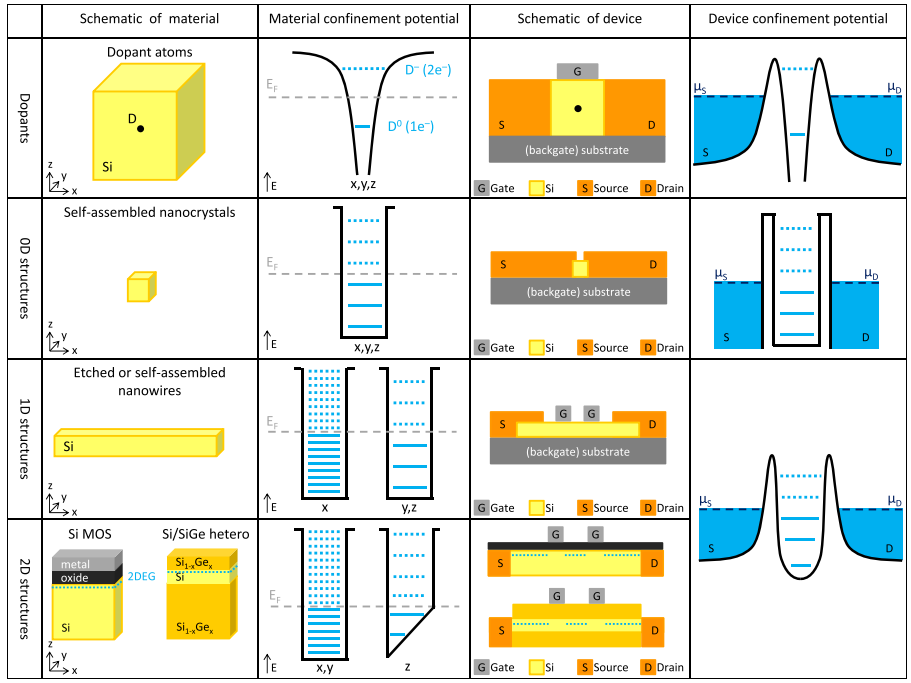
\includegraphics[width = 1\textwidth]{figures/confined_structures_Si.png}
\caption{Sketch of different types of quantum confined structures (image taken from \cite{zwanenburg_silicon_2013})}
\label{fig:confined}
\end{figure}

\subsection{Some numbers}
What's the interaction length-scale for spins? Let's put a few numbers in. Suppose that we want to achieve an (arbitrary) interaction strength of $\sim 10$ kHz, how close should two spins be, in the approximation of dipolar coupling? Dipolar interaction is given by:
\begin{equation}
E = \frac{\mu_0}{4\pi}\frac{ (\hbar \gamma_1) (\hbar \gamma_2)}{r_{12}^3}    
\end{equation}

Let's look at different possibilities:
\begin{enumerate}
    \item for two electron spins ($\gamma_1 = \gamma_2 \sim 2\pi \cdot 28 $GHz/T), , we get a distance $r = 8$ nm.
    \item for an electron spin ($\gamma_1 \sim 2\pi \cdot 28$ GHz/T) and a $^{13}$C nuclear spin ($\gamma_2 \sim 2\pi \cdot 10$ MHz/T), the distance is $r = 1.23$ nm
    \item for two $^{13}$C nuclear spins, the distance is just $0.09$nm!! 
\end{enumerate}

An interaction strength of $10$ kHz means that, under the magnetic field generated by spin-1, spin-2 will take $100 \mu$s to perform a full rotation. It's clear from the numbers above that spin-spin interaction is very localised or, in other words, two spins "feel" each other only when they are very close by! This stems from the weakness of the electron magnetic moment and the very localised $r^{-1/3}$ dependence of the interaction.

As a comparison, the electrostatic (Coulomb) energy between two electrons (charge $-e$) has the form $U_e = k_e (-e)^2/r$. Plugging the numbers in, to achieve an interaction strength $U_e/h$ of $10$ kHz, the distance between the two electrons is as large as $r = 34$m!!!

This has two consequences for quantum devices:
\begin{enumerate}
    \item if you are interested in protecting the quantum state encoded on a spin (for example as a quantum memory), magnetic noise generated by other spins is detrimental only if they are really close to your spin. This means that spins are very protected against noise, provided that the noisy impurities in your device are diluted enough (i.e. the material is of sufficiently high purity)
    \item we will see that one can use a single spin as a sensor. Since such sensor will only detect other particles when they are really close, it will have great spatial resolution. Single spins are therefore a great tool for {\bf nanoscale sensing}
\end{enumerate}


\section {Quantum Spintronics}

\subsection {Spin qubits}
Quantum technologies, such as quantum networks and quantum computers, rely on {\bf qubits} (i.e. quantum bits), the quantum counterpart of a bit. While a classical bit $b$ can take either the value $b=0$ or $b=1$, a qubit can be in a quantum superposition of two pure states, i.e. $\ket{Q} = \alpha \ket{0} + \ket{1}$. This gives a whole range of new properties to be explored and harnessed for new devices. 

Quantum states associated to individual spins can be used as quantum bits for quantum technology. A spin $S=1/2$ can provide an obvious implementation for a qubit, with its two levels $m_s=-1/2$ and $m_s = +1/2$. Higher spins can also implement a qubit, by selecting two of the multiple $m_s$ values available. To implement a qubit, one needs to be able to: (i) initialize; (ii) measure; (iii) manipulate the spin state. In the following sections we will describe how this can be done.

\begin{figure}[h]
\centering
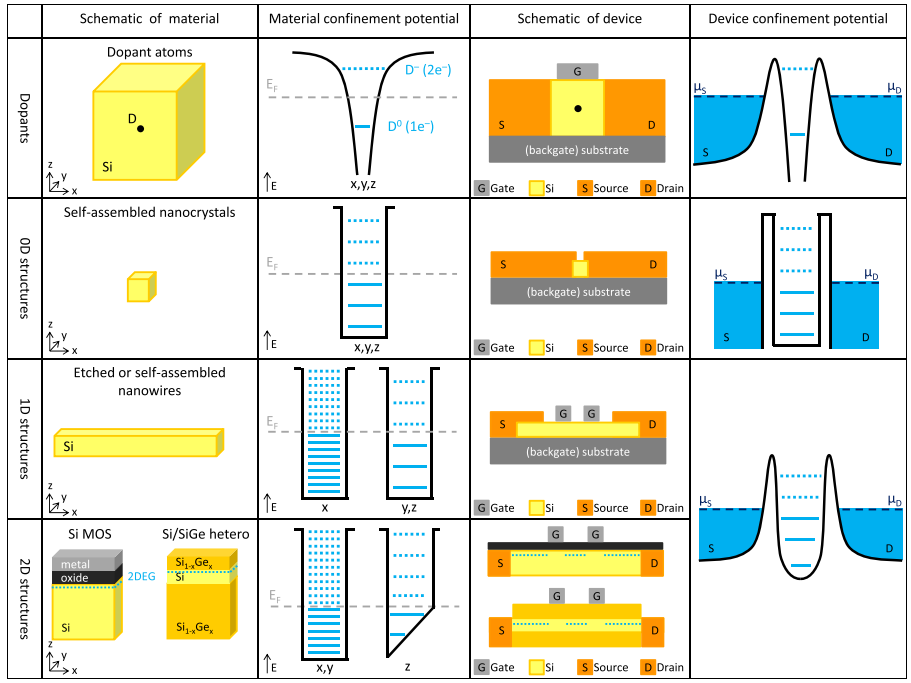
\includegraphics[width = 1\textwidth]{figures/confined_structures_Si.png}
\caption{Examples of implementations of spin qubits: donors in Si (top) and 2DEG quantum dots (bottom). For donors, the confining potential is given by the atomic Coulomb potential, for the quantum dot by electrostatic gates. Image taken from \cite{morton_embracing_2011}}
\label{fig:QD_donor}
\end{figure}

\subsection {Spin qubit platforms}
There are currently several material/device platforms that enable control and detection of individual electronic and nuclear spins. In order to be able to isolate a single electronic spin, a single electron (or a single hole) needs to be spatially confined in a selected portion of space. As you should know from your quantum mechanics classes, spatial confinement (by a "potential well") results in a discretisation of the energy states available to a particle embedded in the well.
\newline We will now briefly discuss two possible approaches to this task.
\subsubsection {Single dopants}
A possible way to create a spin qubit is to exploit a single dopant atom in a crystalline matrix. A widely popular choice, for example, is a $^{31}$P atom in silicon.

The physics of this system is quite similar to the quantum mechanical problem of the hydrogen atom. The electrostatic potential of a single-dopant atom is radially symmetric, resulting in the same steep potential well in all directions, as shown in the first row of Fig. \ref{fig:confined}. The Bohr radius $a_B$ is the mean radius of the orbit of an
electron around the nucleus of an atom in its ground state, and equals, for example, 2.5 nm for $^{31}$P in silicon. A dopant atom can exist in one of three possible charge states: the ionized $D_{+1}$ state (no electron bound to the dopant), the neutral $D_0$ state (one electron bound to the dopant), and the negatively charged $D_{+1}$ state (two electrons bound to the dopant). Because the $D_{+1}$ state corresponds to an empty dopant it does not appear as an electron state in the potential well. 

\subsubsection{Point defects}
Point defects, such an atom missing (vacancy) or an atom replaced by another species, also effectively behave as a single impurity trapped in the solid. The quantum mechanical wavefunction of these systems are very similar to those of a single atom, or a single molecule, but conveniently positioned inside a semiconductor. Experiments on quantum optics mostly rely on a defect in diamond, the nitrogen vacancy centre (consisting of a carbon vacancy with a nearby carbon replaced by a nitrogen atom). This defect is photo-stable even at room temperature (with large phonon sidebands) and it features an $S=1$ electronic spin with excellent coherence properties. Alternative systems for quantum spintronics are spin defects in silicon carbide, such as the Si vacancy or the divacancy.
 
\subsubsection {Self-assembled quantum dots}
Like dopants, self-assembled nanocrystals provide confinement to zero dimensions, but the confinement
is better described by a hard-wall potential well in x, y, and z directions and is much wider (see Fig. \ref{fig:confined}). The energy levels of an electron in a quantum well of size L are quantised according to basic quantum mechanics. The corresponding level spacing $\Delta E$ is on the order of $h^2/m_{eff}L^2$, where $m_{eff}$ is the electron effective mass. The separation between energy levels thus decreases quadratically with the well width: as a result, the discrete levels of, e.g., a
30 nm size nanocrystal are expected to have energy spacings 2 orders of magnitude smaller than those of a dopant with a 3 nm Bohr radius.
\subsubsection {2DEG quantum dots}
A two-dimensional electron gas (2DEG) can be created in MOSFETs and in heterostructures. Electrons are unconfined in the $x$-$y$ plane and are confined by a triangular potential well perpendicular to the plane as sketched in Fig. \ref{fig:confined}.  In a 2DEG-based quantum dot, the lateral confinement is a soft-wall potential defined by top-gate electrodes, enabling tunnel coupling to
source and drain reservoirs in the 2DEG. Those reservoirs are connected to macroscopic wires via Ohmic contacts, which are often highly doped regions at the edge of the chip. The resulting potential landscape is highly tunable thanks to local electrostatic gating via the top gates.

\begin{figure}[h]
\centering
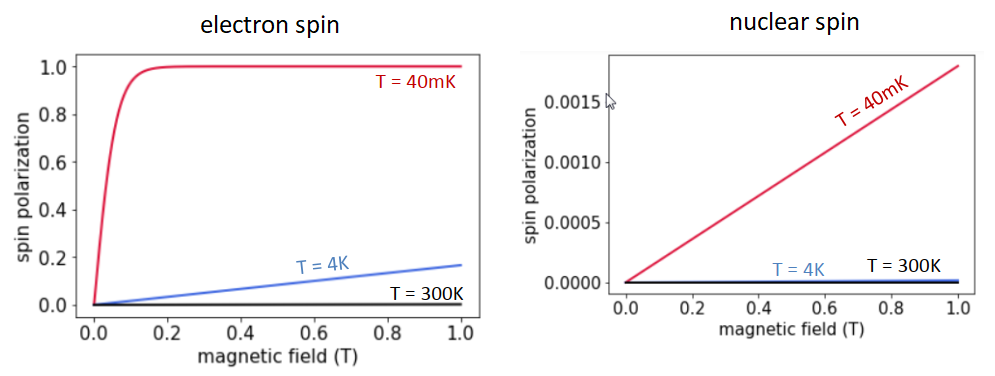
\includegraphics[width = 1\textwidth]{figures/spin_polarisation.png}
\caption{Polarisation $P$ (Eq. AAA) as a function of the applied magnetic field for an electron spin (left) and a $^{13}$C nuclear spin (right), for different temperatures. An electron spin can get effectively fully polarised at mK temperatures for a field of few hundred mT, and it can achieve significant polarisation even at $T=4$K. A nuclear spin, on the other hand, can only achieve minimal polarisation even at ultra-low temperatures.}
\label{fig:spin_polar}
\end{figure}

\subsection {Spin initialisation}
For a two-level system at temperature $T$, statistical mechanics tells us that the probability to be in state $\ket{i}$ is:
\begin{equation}
    p_i = \frac{e^{-E_i/k_BT}}{e^{-E_0/k_BT} + e^{-E_1/k_BT}}
\end{equation}
For a spin $S=1/2$, the energy level are split by the Zeeman effect as $E_{m_s} = \gamma B m_s$. The probability to be in the state $\ket{m_s=-1/2}$ is therefore:
\begin{equation}
    p_{-1/2} = \frac{e^{\gamma B/2 k_BT}}{e^{-\gamma B/2k_BT} + e^{\gamma B/2 k_B T}} = \frac{1}{1 + e^{-\gamma B/k_B T}}
\end{equation}

Therefore, in the limit of very low temperature (compared to the splitting between the energy levels), the probability for the spin to be in the $m_s = -1/2$ state is $100\%$ or, in other words, the spin is polarised into the lower $m_s$ spin sub-level. We can define the {\bf spin polarisation} as:
\begin{equation}
    P = \frac{p_{-1/2}-p_{+1/2}}{p_{-1/2}+p_{+1/2}} = p_{-1/2}-p_{+1/2}
\end{equation}
For temperatures close to zero, when the population is all in $m_s = -1/2$, the spin polarisation is $P = 1$. At high temperature, the probability to be in $m_s=-1/2$ is $50\%$, as the probability to be in  is $m_s=+1/2$. In this case, there is no spin polarisation ($P=0$), and the state is {\bf unpolarised}.
\newline As an example, polarisation for an electron spin as a function of magnetic field is plotted on Fig. \ref{fig:spin_polar} for different temperatures. It can be seen that an electron spin is completely polarised at $T = 40 mK$ at magnetic fields higher then $\sim 200$mT. At $T=4$K, one can achive a $\sim 20\%$ polarisation at a magnetic field of $1$ Tesla (and only weak polarisation at room temperature).  In contrast, for a proton nuclear spin, polarisation is much weaker, given the much smaller Zeeman splitting. This is the reason why high magnetic fields are typically used in MRI medical scans: even in that case, however, the polarisation of the proton spins in your body, at room temperature, will be pretty weak.
\newline For quantum systems used in quantum devices, there are typically other polarisation techniques available, in addition to the application of high magnetic fields at sufficiently low temperature.
\newline {\bf Spin-dependent tunneling.} Consider a quantum dot, modelled as a potential well with finite wall height on one side. Suppose that we apply a strong magnetic field, that induces a considerable Zeeman splitting between the spin states  $\ket{\uparrow}$ and $\ket{\downarrow}$, such that $\ket{\uparrow}$ overcomes the dot energy barrier. At this point, an electron can tunnel out of the dot when in the $\ket{\uparrow}$ state. Therefore, if we start from an unpolarised spin (in $\ket{\uparrow}$ with probability $0.5$ and in $\ket{\downarrow}$ with probability $0.5$), we are only left with an electron when the spin is $\ket{\downarrow}$. Effectively, we have polarised the spin state in $\ket{\downarrow}$.

\begin{figure}[h]
    \centering
    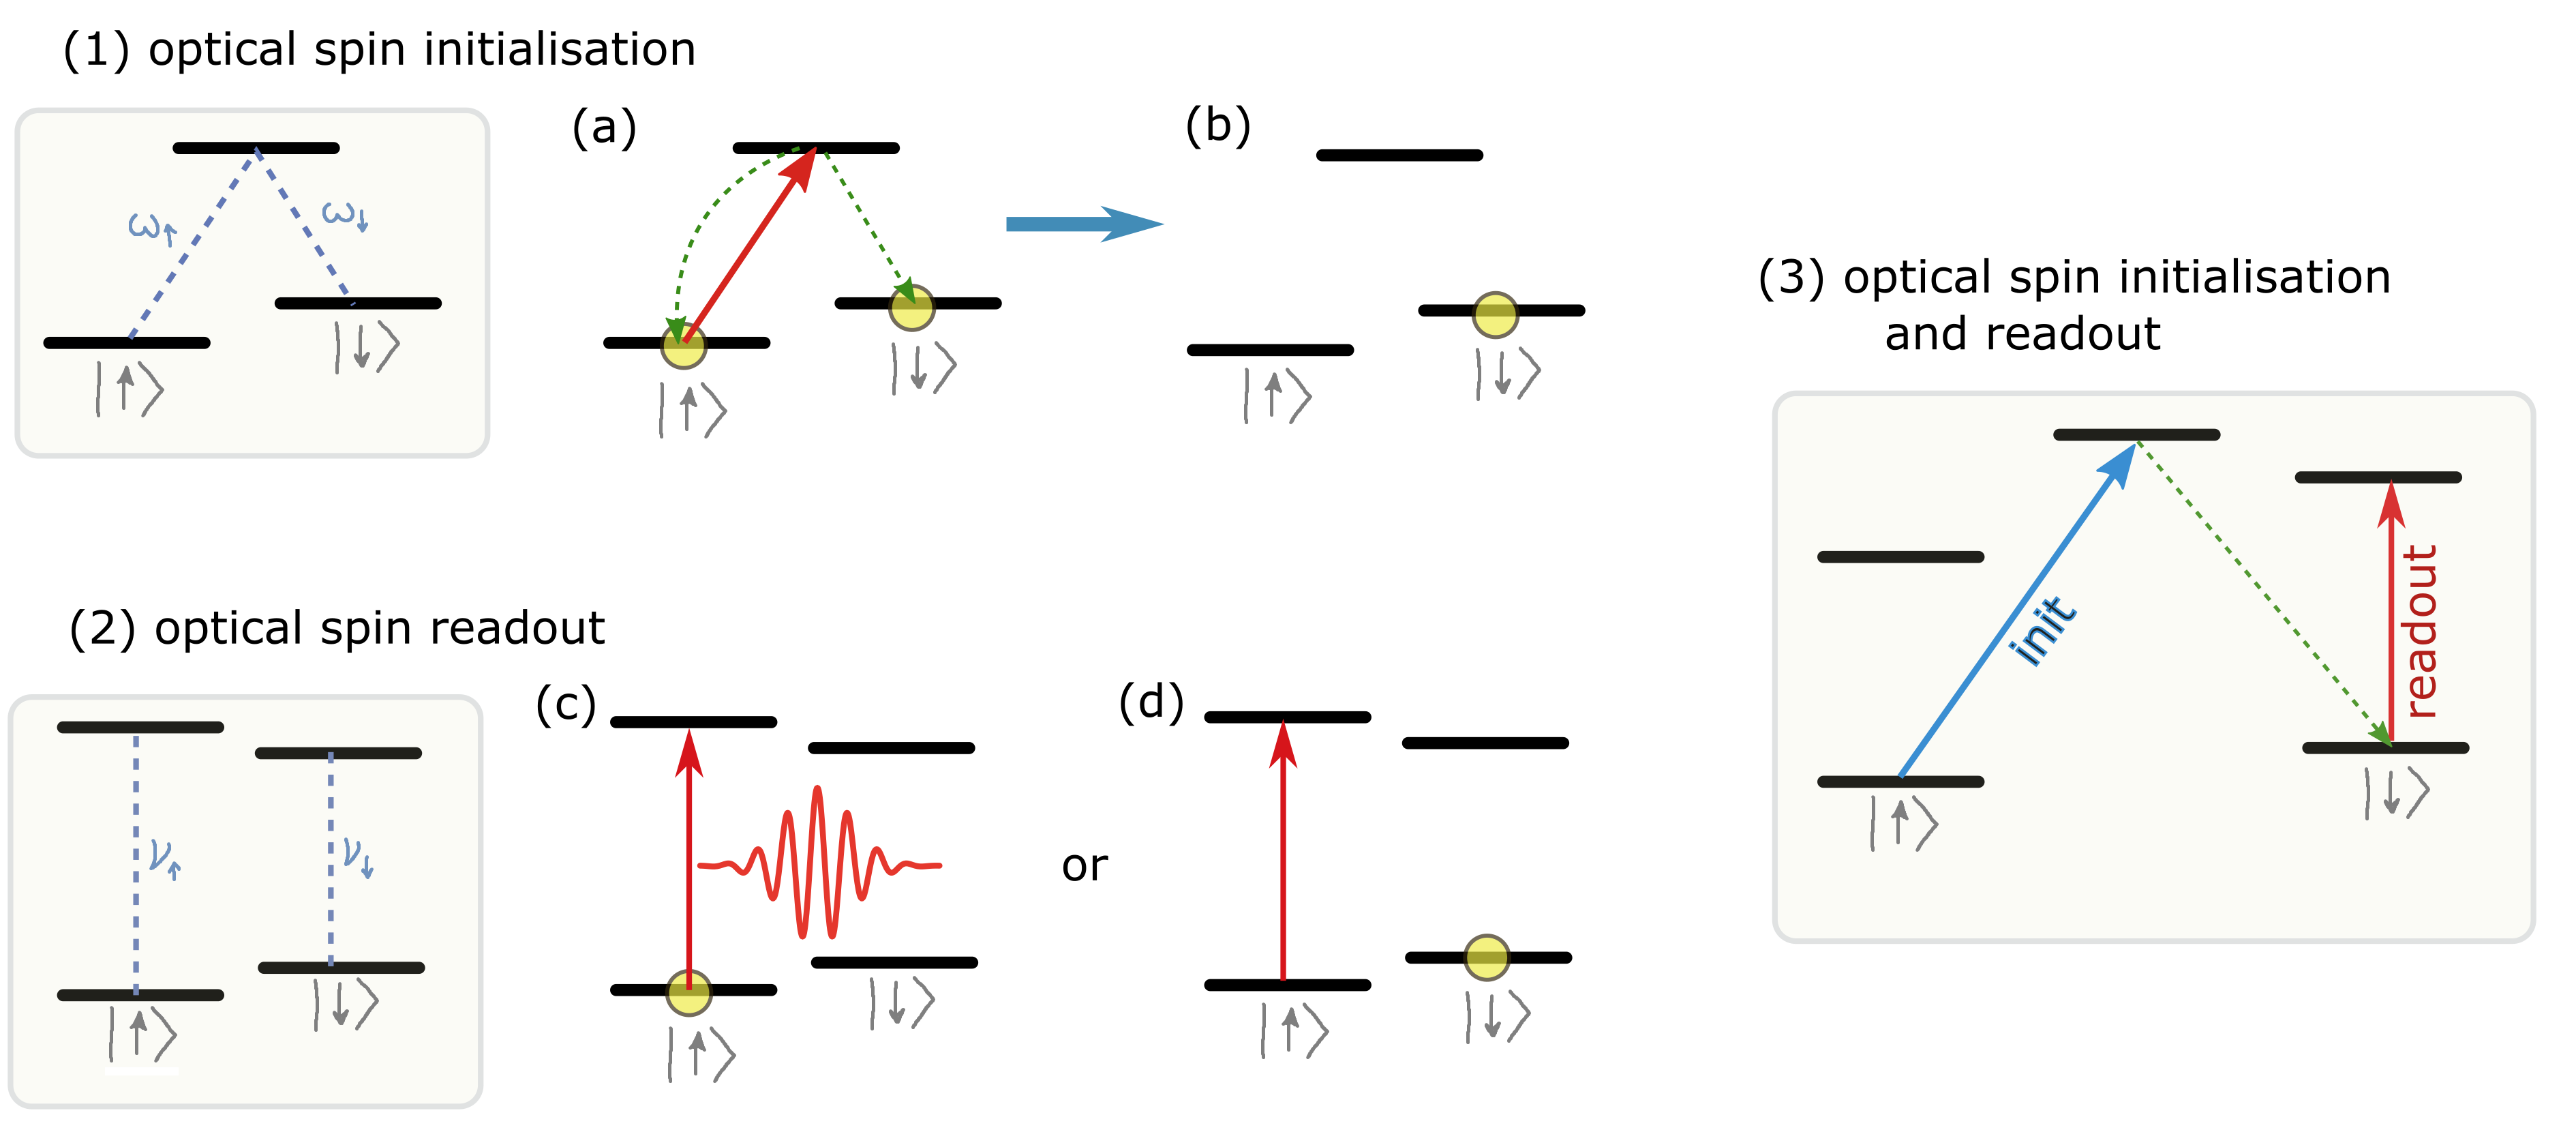
\includegraphics[width =1\textwidth]{figures/optical_spin_init_RO.png}
    \caption{{\bf optical spin polarisation and readout}. {\bf (1)} a $\Lambda$ level system can be efficiently polarise an electronic spin: by exciting the $\omega_{\uparrow}$ "spin-flip" transition between $\ket{\uparrow}$ and the excited state $\ket{e}$ ((a)), the population is pumped out of $\ket{\uparrow}$ and fully transferred to $\ket{\downarrow}$ ((b)). {\bf (2)} two separated "cycling" transitions can be used for spin readout. If the spin state is $\ket{\uparrow}$, selectively exciting the $\nu_{\uparrow}$ transition will generate photons, that can be detected ((c)). If the spin state is $\ket{\downarrow}$, then no photons will be generated when selectively exciting the $\nu_{\uparrow}$ transition ((d)). This scheme relies on the capability to couple to one of the spin states ($\ket{\uparrow}$ in the figure), without exciting the transition $\nu_{\downarrow}$ coupled to $\ket{\downarrow}$. This requires the two optical transitions ($\nu_{\downarrow}$, $\nu_{\uparrow}$) to have different wavelengths, or different optical polarisation. {\bf (3)} a W-scheme, with a combination of "cycling" and "spin-flip" transitions can be used, if available, to achieve both spin polarisation and readout.}
    \label{fig:optical_init_RO}
\end{figure}

{\bf Optical polarisation.} For systems that exhibit atomic-like optical transitions, excitation of spin-selective optical transitions by narrowband laser light can enable initialisation of the spin state. Consider, for example, the energy level scheme in Fig. \ref{fig:optical_init_RO}: this is known as a $\Lambda$-system due to its structure. We have two ground states, one labeled as $\ket{\uparrow}$ and the other as $\ket{\downarrow}$, coupled to a common excited state $\ket{e}$. The energy splitting $E_{\uparrow}$ between the $\ket{\uparrow}$ ground state and the excited state $\ket{e}$, is different than the  energy splitting $E_{\downarrow}$ between the $\ket{\downarrow}$ ground state and the excited state $\ket{e}$. Therefore the frequencies of the two transitions are different and one can selectively excite one of the two, coupling only to one specific ground state.
\newline Let us suppose that the ground state is unpolarised (i.e. in $\ket{\uparrow}$ with probability $0.5$ and in $\ket{\downarrow}$ with probability $0.5$). Let us shine a laser with frequency $\omega_{\uparrow} = E_{\uparrow}/\hbar$. If the system is in the $\ket{\uparrow}$ state, excitation brings it to the excited state $\ket{e}$, from which it can decay either back to $\ket{\uparrow}$ or to $\ket{\downarrow}$. If it decays back to $\ket{\uparrow}$, it is just re-excited again by the laser. If it decays to (or starts from) $\ket{\downarrow}$, the laser light does not couple to the transition to the excited state, since the frequency is different (now we would need a laser tuned at $\omega_{\downarrow} = E_{\downarrow}/\hbar$. In this case, the population is just "stuck" in $\ket{\downarrow}$ and a laser tuned at $\omega_{\uparrow}$ cannot bring the system out of $\ket{\downarrow}$. Therefore, eventually, the system gets initialised in the $\ket{\downarrow}$ state with high fidelity.
\newline This scheme can work also with energy levels not necessarily in a $\Lambda$ structure, sometimes for example one of the transitions (for example $\omega_{\downarrow}$) is only weakly allowed: optical polarisation still works, albeit at slower rates.

\begin{figure}[h]
\centering
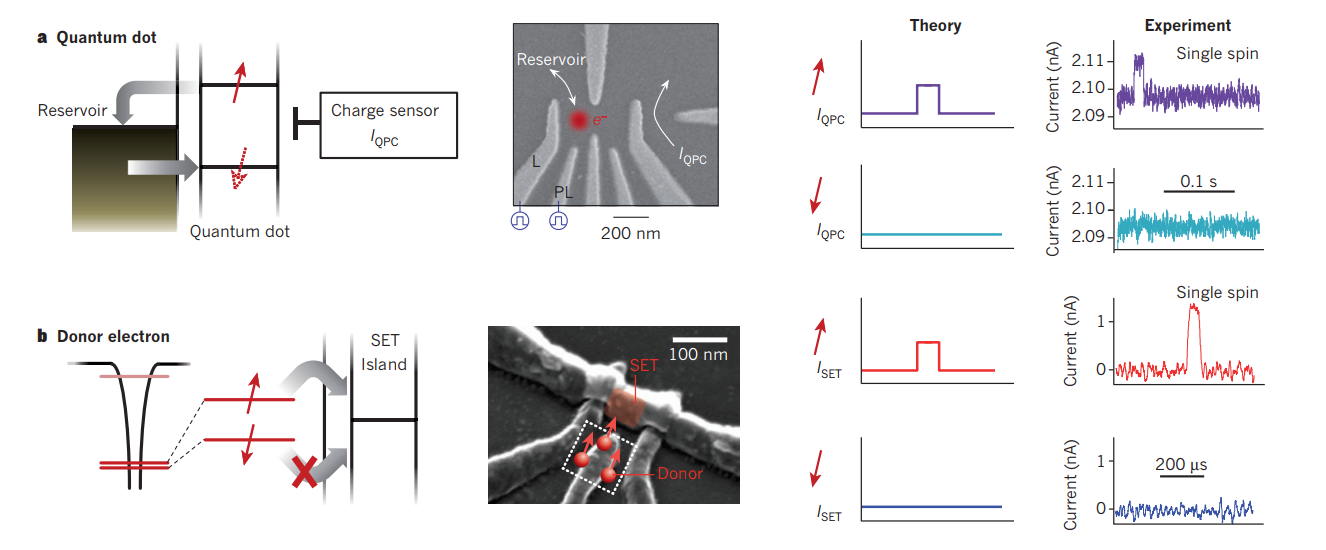
\includegraphics[width = 1\textwidth]{figures/QD_donor_readout.png}
\caption{ {\bf Electrical spin readout mechanisms} from \cite{morton_embracing_2011}. {\bf(a)} on the top row, readout scheme for an electrostatic 2DEG quantum dot, through spin-dependent tunneling rates. The two spin states for a single electron are split by a magnetic field, such that the $\ket{\uparrow}$ state has sufficient energy to tunnel out of the dot. A charge sensor detects the charging state of the dot, as shown by the experimental data on the right. {\bf (b)} on the bottom row, a similar scheme outline for a donor in silicon, coupled to a single electron transistor for charge detection.}
\label{fig:QD_RO}
\end{figure}

\subsection {Spin detection}
Given that the magnetic moment of a single electron ($\mu_B$) is tiny, it is very challenging to detect it directly. In quantum devices, spin detection is performed by exploiting the correlation of the spin state with other degrees of freedom, resulting from the device physics (in a similar way as we have described for spin polarisation):
\newline {\bf Spin-to-charge conversion.} This protocol works by converting the spin state (corresponding to a tiny magnetic moment, hard to measure) into a charge (or current), which is much easier to detect. For example, one can use the same idea of spin-dependent tunneling as above, but coupling the quantum dot to a single-electron charge sensor (for example a single electron transistor) or to an amplifier and current meter capable of detecting extremely faint currents. Following the example above, if the spin is in the $\ket{\uparrow}$ state, the electron can tunnel out of the dot, so that the charge sensor can discriminate a change in the charge state trapped in the dot. Or, one can detect the tiny current arising from the electron tunneling out of the dot.
\newline Spin-to-charge conversion can also be accomplished optically, by shining a strong laser tuned to a frequency that only couples to one specific spin state. If the system is ionised (i.e. the electron is optically ejected), one can then detect a difference in the charge state. This can be performed, as above, with a single-electron transistor, or it can lead to a detectable change in the optical emission properties of the system (for example a change in the photo-luminescence spectrum).
\newline {\bf Optical spin detection}. The physics behind optical spin detection is quite similar to what we discussed for optical spin polarisation, only based on a different energy level structure. Please consider the energy level scheme in Fig \ref{fig:optical_init_RO}. Again, we have two ground states ($\ket{\uparrow}$ and $\ket{\downarrow}$), but they are now coupled to two different excited states ($e_{\ket{\uparrow}}$ and $e_{\ket{\downarrow}}$, respectively. The corresponding optical transition frequencies are, again, distinct ($\tilde{\omega}_{\uparrow}$ and $\tilde{\omega}_{\downarrow}$). If the spin is in the $\ket{\uparrow}$ and we apply a laser at frequency $\tilde{\omega}_{\uparrow}$, then the system is promoted to the excited state and decays back emitting a photon. On the other hand, if the spin is in the $\ket{\downarrow}$ and we apply a laser at frequency $\tilde{\omega}_{\uparrow}$, the laser cannot bring the system to the excited state because the frequency is off and no photon is emitted. Therefore, by shining a laser at frequency $\tilde{\omega}_{\uparrow}$ and detecting whether photons have been emitted or not, we can measure the spin state: if photons are emitted, the spin state was $\ket{\uparrow}$, otherwise the spin state was $\ket{\downarrow}$.

\subsubsection{Single-shot vs averaged readout}
As we have seen, given ghat the detection of the magnetic moment of a single electron is very complicates, most spin detection scheme rely on converting the spin state into a charge or a photon intensity, which are much easier to measure. This conversion associates to each of the two spin states ($\ket{\uparrow}$ and $\downarrow$), a number $x_{\uparrow}$ or $x_{\downarrow}$ of electrons or photons. Given the discrete nature of electrical charge and photon intensity, these values are limited by shot (Poissonian noise). We can distinguish two operation regimes:
\begin{enumerate}
    \item {\bf single-shot readout}. In this case, the difference between $x_{\uparrow}$ and $x_{\downarrow}$ is larger than the widths of the distributions, so one can reliably determine the spin state by the number of detected events. This means that optical excitation or spin-to-charge conversion gives enough photons or electrons that we can reliably determine the spin state.
    \item {\bf averaged readout}. In some case, the difference between $x_{\uparrow}$ and $x_{\downarrow}$ is smaller than the widths of the distributions. This happens because the readout process itself flips the spin after some time, and therefore we cannot accumulate enough statistics to reliably determine the spin state by the number of detected events. In this case, the only possibility is to repeat the experiment many times (thereby, the "averaging"), until sufficient statistics is accumulated.
\end{enumerate}

\begin{figure}[h]
\centering
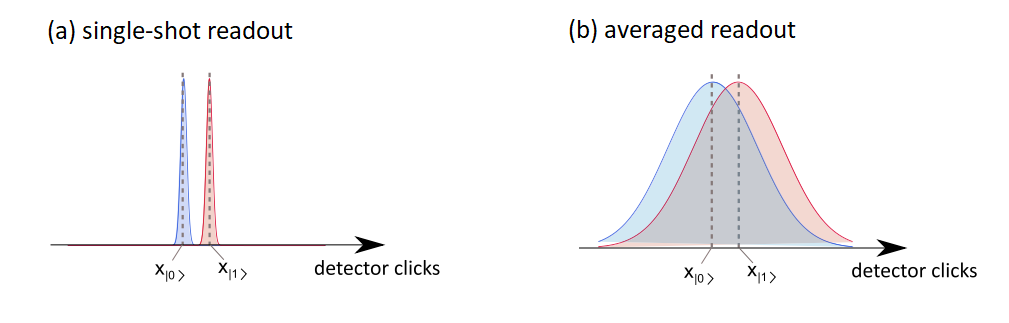
\includegraphics[width = 0.8\textwidth]{figures/readout_SSRO_AVG.png}
\caption{Readout of a qubit $\ket{Q} = \alpha \ket{0} + \beta \ket{1}$ delivers a different number of events ($x_0$ or $x_1$), e.g. detected photons or electrons, depending on the readout basis state ($\ket{0}$ or $\ket{1}$). If the difference in detector clicks between $x_0$ and $x_1$ is larger than their standard deviation, then the qubit state can be determined in a {\bf single shot}. Otherwise, several repetions needs to be performed to infer the qubit state ({\bf averaged readout}). }
\label{fig:SSRO}
\end{figure}



\subsection {Spin relaxation}
At finite temperature, once a spin system has been polarised, it does not hold polarisation forever, but it tends to relax a thermal-equilibrium {\it "un-polarised"} distribution. In magnetic resonance terminology, the time for a polarised spin system to reach a thermal equilibrium distribution is known as $T_1$ {\it (longitudinal) spin relaxation time} or {\it spin-lattice relaxation time}. In spin systems, relaxation does not typically happen for direct decay (like an excited atoms decays to the ground state emitting a photon): these timescales are extremely long.

\begin{figure}[h]
\centering
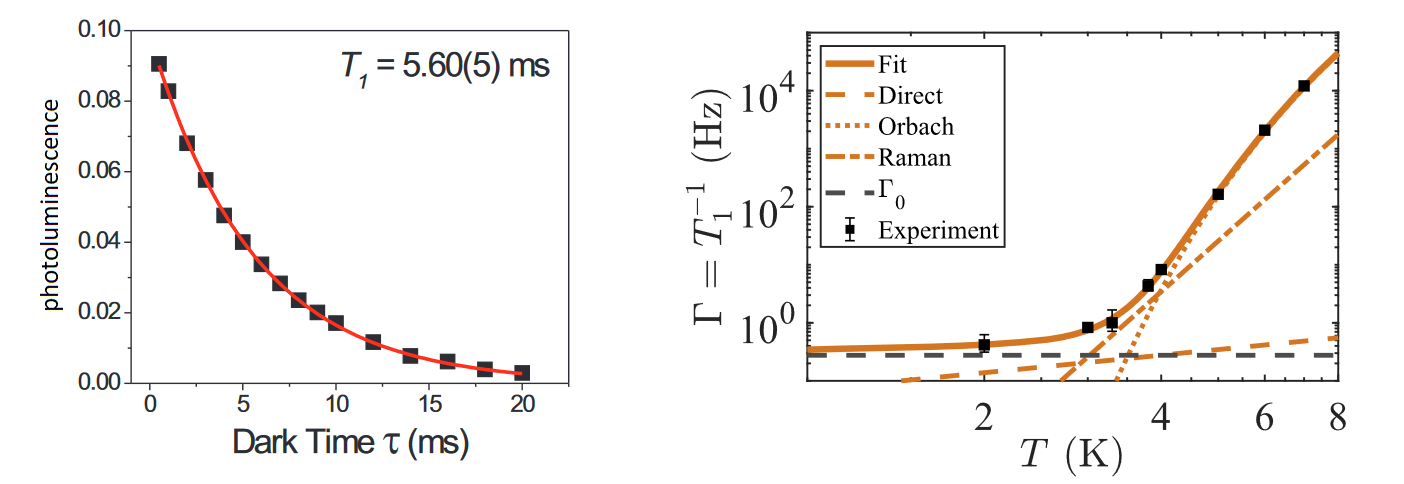
\includegraphics[width = 1\textwidth]{figures/T1_example.png}
\caption{{\bf $T_1$ relaxation}. On the left, experimental measurement of $T_1$ relaxation for the electronic spin of a nitrogen-vacancy centre in diamond, at room temperature (with characteristic $e^{-\tau/T_1}$ dependence. On the right, experimental data for the relaxation rate ($1/T_1$) for Mo impurities in SiC, as a function of the temperature $T$, highlighting the impact of the different spin-phonon processes that affect relaxation (from \cite{gilardoni_spin-relaxation_2020}).}
\label{fig:T1_exp}
\end{figure}


The main relaxation mechanism for relaxation of spins in quantum devices is coupling to electrics fields. In principle, electric fields cannot cause direct transitions between pure spin states. However, we have seen that the spin-orbit
interaction perturbs the spin states and the eigenstates become admixtures of spin and orbital states. These new eigenstates can be coupled by electric fields, and electric-field fluctuations can lead to spin relaxation. In general, fluctuating electric fields could arise from
many sources, including fluctuations in the device gate potentials (if any), background charge fluctuations or other electrical
noise sources However, if the device and the measurement system are design carefully, the
electric-field fluctuations of these external noise sources is less important than those caused by the phonon bath. Phonons can produce electric-field fluctuations in two ways. First, phonons inhomogeneously deform the crystal lattice, altering the band gap in space, which gives rise to fluctuating electric fields. This mechanism occurs in all semiconductors. Second, in polar crystals such as GaAs, also homogeneous strain leads to electric fields, through the piezoelectric effect.


Spin relaxation typically is driven by three different processes, which can be experimentally distinguished by a different dependence of $T_1$ on the temperature $T$:
\begin{itemize}
    \item {\bf direct} photon absorption/emission ($1/T_1 \propto T$). There is an exact match of the spin transition energy with a phonon energy so there can be direct transfer of energy from the spin system to the lattice phonon bath, involving the collective motion of lattice atoms.
    \item {\bf Raman} phonon scattering ($1/T_1 \propto T^7$ or $T^9$). This is a two-phonon process in which the energy to be transferred to the lattice is the difference between the energies absorbed and emitted for a virtual excited state at any energy less than the Debye temperature.
    \item {\bf Orbach} processes ($1/T_1 \propto e^{-\Delta/k_B T}$). This is a two-phonon process in which the energy to be transferred to the lattice is the difference between the energies absorbed and emitted for a specific low-lying excited state.
\end{itemize}

Typically, a $T_1$ measurement is performed as follows:
\begin{enumerate}
\item the spin is initialised in $\ket{\uparrow}$
\item we wait a time $\tau$ 
\item the spin state is measured.
\end{enumerate}
When plotting the probability to be in the state $\ket{\uparrow}$ as a function of $\tau$ one gets an exponential decay as:
\begin{equation}
    P_{\ket{\uparrow}} \sim \frac{1 + e^{-\tau/T_1}}{2}
    \label {eq:T1}
\end{equation}

\subsection {Rabi oscillations}
Let us consider a two-level system (represented by the Hamiltonian $(\omega_0/2)\hat{\sigma}_z$, for example corresponding to a spin $S=1/2$ system with a magnetic field applied along the $z$ direction. Let's suppose to apply an oscillating magnetic field along the $x$ direction, with frequency $\omega$, amplitude $\Omega$ and phase $\varphi$:

\begin{equation}
    \hat{\mathcal{H}} = \frac{\omega_0}{2}\hat{\sigma}_z + \Omega \mbox{cos} \left ( \omega t + \varphi \right) \hat{\sigma}_x
\end{equation}
In this equation, and throughout the whole section, we will take $\hbar = 1$ to simplify the notation. This is a time-dependent Hamiltonian, so the dynamics cannot be solved by easily diagonalising the time-independent Schroedinger equation.
\newline Let us move to a {\bf rotating frame} which rotates at angular frequency $\omega$ around the $z$ axis. A rotation at $\omega$ on the $X-Y$ plane (cos$(\omega t + \varphi)$) can be decomposed in two terms, one at angular frequency $+\omega$ ($e^{i \omega t}$) and one at angular frequeny $-\omega$ ($e^{-i \omega t}$). Intuitively, if you set yourself in a frame rotating with angular frequency $\omega$ around the $z$ axis, you will see the $+\omega$ component moving together with you (i.e. at angular frequency $0$ with respect to you), and the $-\omega$ component moving away from  you at angular frequency $-2\omega$.
\newline Formally, transforming the Hamiltonian to a frame rotating at angular frequency $\omega'$ around the $z$ axis is achieved by the operator:
\begin{equation}
    \hat{U} = e^{i \frac{\omega' t}{2} \hat{\sigma}_z}
\end{equation}
When applied to the system state $\ket{\psi}$: $\hat{U} \ket{\psi} = \ket{\Phi}$.
Multiplying Schroedinger's equation on the left by $\hat{U}$ and with some algebra (please check it yourself), one gets a new Schroedinger equation for the state in the rotating frame $\ket{\Phi}$, with the transformed Hamiltonian in the rotating frame being:
\begin{equation}
    \widetilde{\mathcal{H}} = U \hat{\mathcal{H}} U^{\dagger} - i \hbar U \frac{d\hat{U}^{\dagger}}{dt}
\end{equation}
\newline What does this Hamiltonian correspond to? With some algebra (please work it out yourself), we find that:
\begin{equation}
    U \sigma_z U^{\dagger} = \sigma_z
\end{equation}
\begin{equation}
    U \sigma_x U^{\dagger} = \cos(\omega' t) \sigma_x - \sin(\omega' t) \sigma_y 
\end{equation}
\begin{equation}
    U \sigma_y U^{\dagger} = \sin(\omega' t) \sigma_x + \cos(\omega' t) \sigma_y
\end{equation}
\begin{equation}
    U \frac{dU^{\dagger}}{dt} = -i \frac{\omega'}{2}\sigma_z
\end{equation}
Using these results, we get:
\begin{equation}
    \widetilde{\mathcal{H}} = \frac{\omega_0-\omega'}{2}\hat{\sigma}_z + \frac{\Omega}{2} \alpha_+ + \frac{\Omega}{2} \alpha_-
\end{equation}
where:
\begin{equation}
\label{eq:alpha}
    \alpha_{\pm} = \cos \left[ \left( \omega \mp \omega'  \right)t + \varphi \right] \hat{\sigma}_x \pm \sin \left[ \left( \omega \mp \omega'  \right)t + \varphi \right] \hat{\sigma}_y
\end{equation}
Assuming now that the rotating frame angular velocity $\omega'$ is the same as for the electromagnetic excitation (i.e. $\omega' = \omega$), then Eq. \ref{eq:alpha} simplifies to:
\begin {equation}
\alpha_+ = \cos \varphi \hat{\sigma}_x +  \sin \varphi \hat{\sigma}_y
\end{equation}
and:
\begin{equation}
    \alpha_- = \cos \left( 2 \omega t + \varphi \right) \hat{\sigma}_x - \sin \left( 2\omega + \varphi \right) \hat{\sigma}_y
\end{equation}
As described intuitively above, the Hamiltonian features two terms, one static with no time dependence (moving together with the observer in the rotating frame) and one moving away from the observer rotating frame at frequency $-2 \omega$.

We can now take one more assumption, the so-called {\bf rotating wave approximation (RWA)}. This approximation states that the fast oscillating term at $2 \omega$ is effectively averaged out so that only the static term really contributes to the dynamics. This allows us to simplify the Hamiltonian and to reduce it to a time-dependent Hamiltonian, that we know how to solve:
\begin{equation}
 \widetilde{\mathcal{H}} = \frac{\omega_0-\omega}{2}\hat{\sigma}_z + \frac{\Omega}{2} \cos\varphi \hat{\sigma}_x + + \frac{\Omega}{2} \sin\varphi \hat{\sigma}_y 
\end{equation}
\newline This Hamiltonian is, mathematically, identical to the strong-coupling Hamiltonian we discussed in B21NT (Nanophotonics), for those of you who have taken that course. In the following, we will be going through exactly the same derivation.
\newline The Hamiltonian can be written in matrix form as:
\beq
\label{eq:rabi_H}
\mathcal{H} = \frac{1}{2}\left(\begin{array}{cc}
\Delta & \Omega\\
\Omega^* & -\Delta
\end{array} \right)
\eeq
where the $\Delta$ is detuning between the exciting electromagnetic field and the atomic resonance ($\Delta = \omega_0 - \omega$). 
This matrix is diagonalised by the eigenvalue equation:
\begin{equation}
 (\widetilde{\omega} - \Delta)^2 - |\Omega|^2=0
 \end{equation}
which gives the solution:
\begin{equation}
\label{eq:rabi_frq}
 \widetilde{\omega}_{1/2} = \sqrt{\Delta^2 + |\Omega|^2 }
\end{equation}

In the case of {\bf resonant excitation} (i.e. $\Delta = 0$), a quantum state initialised in $\ket{\downarrow}$ will oscillate as:
\begin{equation}
\label{eq:rabi_evol}
 \ket{\psi (t)} \propto  e^{-i |\Omega| t/2} \ket{\downarrow} + e^{i |\Omega| t/2} \ket{\uparrow}
\end{equation}
Physically, this means that the system coherently  cycles between the two spin states. The oscillations are called {\bf Rabi oscillations}. In Nanophotonics, when discussing strong-coupling we talked about ''vacuum`` Rabi oscillations because the oscillations were not induced by any electromagnetic driving. Here, instead, we do have a driving electromagnetic field. 
\newline The driving amplitude $|\Omega|$ determines the frequency of the oscillations: the larger $|\Omega|$ the faster the oscillations, for $|\Omega| \rightarrow 0$ the oscillations become slower and slower.

In case where the driving field in {\bf non-resonant} (i.e. $\Delta \neq 0$), the frequency of the Rabi oscillations is modified as in Eq. \ref{eq:rabi_frq}. In this case, the frequency of the Rabi oscillations increases with the detuning $\Delta$. In other words, if you drive a $S=1/2$ spin on resonance with an amplitude $|\Omega|$, the spin will rotate with Rabi frequency $|\Omega|$.
If your driving field is detuned from the Zeeman splitting $\omega_0$ between the energy levels $m_s = -1/2$  ($\ket{\downarrow}$) and $m_s = +1/2$ ($\ket{\uparrow}$), then the rotation frequency will increase as $\sqrt{|\Omega|^2+(\omega_0 - \omega)^2}$ 

\begin{figure}[h]
    \centering
    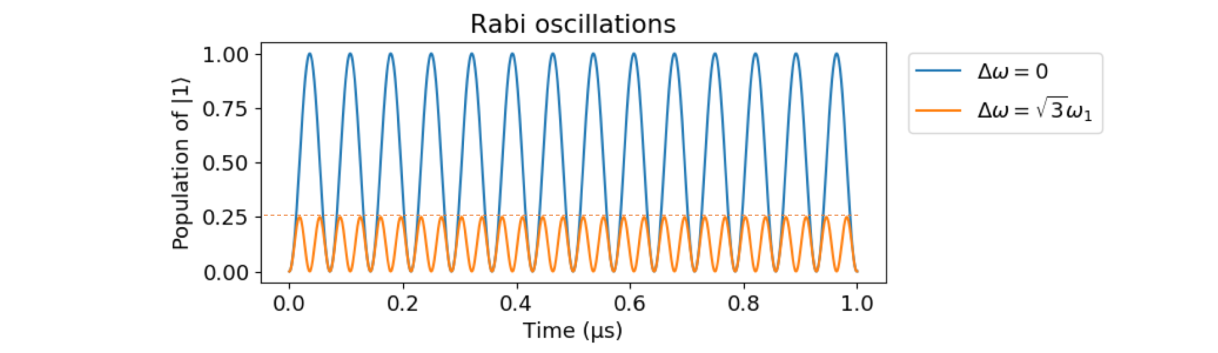
\includegraphics[width =1\textwidth]{figures/rabi.png}
    \caption{Rabi oscillations on a two-level system, driven by (a) resonant excitation ($\Delta = 0$) - (b) with a detuning. Excitation at a detuned frequency results in Rabi oscillations with larger frequency and smaller amplitude.}
    \label{fig:rabi}
\end{figure}


\subsection{Spin state preparation}
Let us now go back to the eigenvalue equation for Eq. \ref{eq:rabi_H} and examine more carefully how this affect the evolution of a spin state. Computing the matrix eigenvectors (please work it out yourself), one finds:
\begin{subequations}
\begin{align}
\ket{\psi_+}&=e^{-i\varphi/2} \cos{\left( \frac{\theta}{2}\right)} \ket{\downarrow} + e^{i\varphi/2} \sin{\left(\frac{\theta}{2}\right)} \ket{\uparrow}\\
\ket{\psi_-}&=-e^{-i\varphi/2} \sin{\left( \frac{\theta}{2}\right)} \ket{\downarrow} + e^{i\varphi/2} \cos{\left(\frac{\theta}{2}\right)} \ket{\uparrow}
\end{align}
\end{subequations}
Here $\varphi$ is the phase of the driving electromagnetic field and:
\begin{equation}
    \tan{\theta} = \frac{|\Omega|}{\Delta}
\end{equation}
As usual for the time-independent Schroedinger equation, any quantum state $\ket{\Phi}$ shall be expressed in the basis vectors of the eigenvectors $\lbrace \ket{\psi_+}, \ket{\psi_-} \rbrace$ of the Hamiltonian in Eq. \ref{eq:rabi_H} and then each will evolve picking up a relative phase proportional to the corresponding eigenvalues.

For example, suppose we initially prepared the spin state $\ket{\downarrow}$ (i.e $m_s = -1/2)$. This can be expressed in terms of the eigenvectors $\lbrace \ket{\psi_+}, \ket{\psi_-} \rbrace$ as:
\begin{equation}
\begin{split}
    \ket{\downarrow}& = \braket{\psi_+}{\downarrow}  \ket{\psi_+} + \braket{\psi_-}{\downarrow}  \ket{\psi_-}\\
    &= e^{-i\varphi/2} \cos{\left( \frac{\theta}{2}\right)}\ket{\psi_+} - e^{i\varphi/2} \sin{\left( \frac{\theta}{2}\right)}\ket{\psi_-}
\end{split}
\end{equation}

The evolution of the quantum state as a function of the time $t$ over which the driving field is applied can be written as:
\begin{equation}
    \ket{\Phi (t)} = e^{-i\varphi/2} \cos{\left( \frac{\theta}{2}\right)} e^{i\sqrt{|\Omega|^2+\Delta^2}t/2}\ket{\psi_+} - e^{i\varphi/2} \sin{\left( \frac{\theta}{2}\right)}e^{-i\sqrt{|\Omega|^2+\Delta^2}t/2}\ket{\psi_-}
\end{equation}
Depending on the diving parameters ($\Delta$, $\Omega$ and $t$), one can control the spin state $\ket{\Phi (t)}$ over time.

Let us for the moment neglect the phase $\varphi$ of the drive. The probability for the spin to be found in the state $\ket{\uparrow}$ is given by:
\begin{equation}
\begin{split}
    P_{\ket{\uparrow}}(t) &= |\braket{\uparrow}{\Phi(t)}|^2\\
    &= \left| \sin{\frac{\theta}{2}}\cos{\frac{\theta}{2} \left(e^{-i\frac{t}{2}\sqrt{|\Omega|^2+\Delta^2}} - e^{i\frac{t}{2}\sqrt{|\Omega|^2+\Delta^2}} \right)}\right|^2\\
    &= \frac{|\Omega|^2}{|\Omega|^2+\Delta^2} \sin^2{\left( \frac{t\sqrt{|\Omega|^2+\Delta^2}}{2}\right)} \label{eq:rabi_final}
\end{split}
\end{equation}

Eq. \ref{eq:rabi_final} is very important, and it tells us several things:
\begin{itemize}
    \item as we have seen before the frequency of the Rabi oscillations is minimal for resonant driving ($\Delta = 0$) and increases when a detuning is present as $\frac{\sqrt{|\Omega|^2+\Delta^2}}{2}$.
    \item the amplitude of the Rabi oscillations, given by $\frac{|\Omega|^2}{|\Omega|^2+\Delta^2}$, achieves $100\%$ contrast for resonant driving. When $\Delta \neq 0$, the amplitude of the Rabi oscillations between $\ket{\downarrow}$ and $\ket{\uparrow}$ decreases. 
\end{itemize}

\subsubsection{Useful control pulses: $\pi$ and $\pi/2$ pulses}
We have seen above that controlling the duration of time (let's call it $\Delta t$) over which we apply a driving electromagnetic field, together with its amplitude $\Omega$ and the detuning $\Delta$, can prepare arbitrary spin states.

Let us assume we are driving the spin on resonance ($\Delta = 0$). There are two types of excitation pulses that are widely used for the control of quantum devices:
\begin{itemize}
    \item a {\bf $\pi$ pulse} is a pulse of duration $\Delta t$ such that $|\Omega| \Delta t = \pi$. In this case, according to Eq. \ref{eq:rabi_final}, the spin state is switched from $\ket{\downarrow}$ to $\ket{\uparrow}$ (or viceversa).
    \item a {\bf $\pi/2$ pulse} is a pulse of duration $\Delta t$ such that $|\Omega| \Delta t = \pi/2$. Using a $\pi/2$ pulse, one can, starting from $\ket{\downarrow}$, prepare an equal superposition state:
    \begin{equation}
        \ket{Q} = \frac{\ket{\downarrow} + \ket{\uparrow}}{\sqrt{2}}
    \end{equation}
\end{itemize}

One thing to note is that, even though we have not really discussed it here, there is one additional knob available for state preparation, i.e. the phase $\varphi$ of the drive. This parameter control the rotation axis, e.g. one could decide to apply a $\pi$ pulse around $x$ or around $y$, etc.


\begin{figure}[h]
\centering
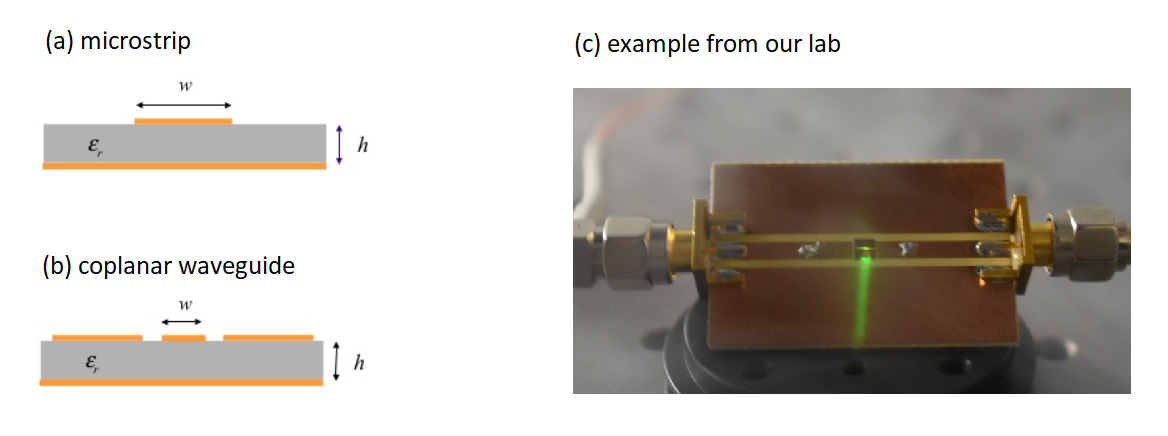
\includegraphics[width = 1\textwidth]{figures/microwaves.png}
\caption{Examples of structures to deliver a microwave magnetic field for spin driving. {\bf (a)} microstrip. {\bf (b)} coplanar waveguide. All structures need to be design for $50 \Omega$ impedance at the operation frequency to avoid reflections and pulse distortion. {\bf (c)} Example from our lab. Microwaves are delivered to the sample via a coaxial cable (with SMA connector), through a coplanar waveguide and then a thin ($20 \mu$m) wire soldered across the diamond sample.}
\label{fig:MW}
\end{figure}



\subsubsection{Experimental considerations}
For an electron spin ($\gamma_e \sim 28 $GHz/T for magnetic fields in the $~100$mt-$1$T range, the Zeeman splitting is on the GHz range, i.e. the two-level system needs to be driven by microwave frequencies. For nuclear spins, the gyromagnetic ratio is $\sim 10^3$ times smaller, leading to driving fields in the radio-frequency rang (MHz frequencies).
\newline Experimentally, this means that spin manipulation require some careful radio-frequency/microwave engineering to deliver the required oscillating magnetic field with high efficiency and fidelity to the spin. This can be done by several types of antennas:
\begin{itemize}
    \item when applying a current $I$ to a wire, from Biot-Savart's law the resulting magnetic field $B(R)$ at a distance $R$ is:
    \begin{equation}
        B(R) = \frac{\mu_0 I}{2 \pi R} 
    \end{equation}
    The magnetic field $B$ is tangential on circles around the wire. An ac magnetic field in the GHz range can be generated by applying an ac current at the corresponding frequency.
    
    \item an alternative could be a coil, either an external coil with multiple loops, or a single-coil loop directly deposited on-chip. For a coil with $N$ loops for a length $L$, driven by a current $I$:
    \begin{equation}
        B = \mu_0 \frac{N}{L} I
    \end{equation}
    
    \item a planar microwave structure, such as a coplanar waveguide or a microstrip waveguide. These structures operate with small losses over a broad frequency range, and can be designed for $50 \Omega$ impedance to minimise reflections that would deform the shape of the microwave pulses applied to the spin system
    
    \item resonant antennas, based on a structure with inductance $L$ and capacitance $C$ optimised such that the desired resonance frequency is $\omega_0 = 1/\sqrt{LC}$. A resonant antenna will only operate at frequencies close to $\omega_0$, with the bandwidth determined by the quality factor $Q$ of the circuit. A resonant antenna can boost the microwave power by a factor $Q$, which is important when low microwave power needs to be applied (for example when operating at cryogenic temperature with limited cooling power, to avoid heating)
\end{itemize}

\begin{figure}[h]
\centering
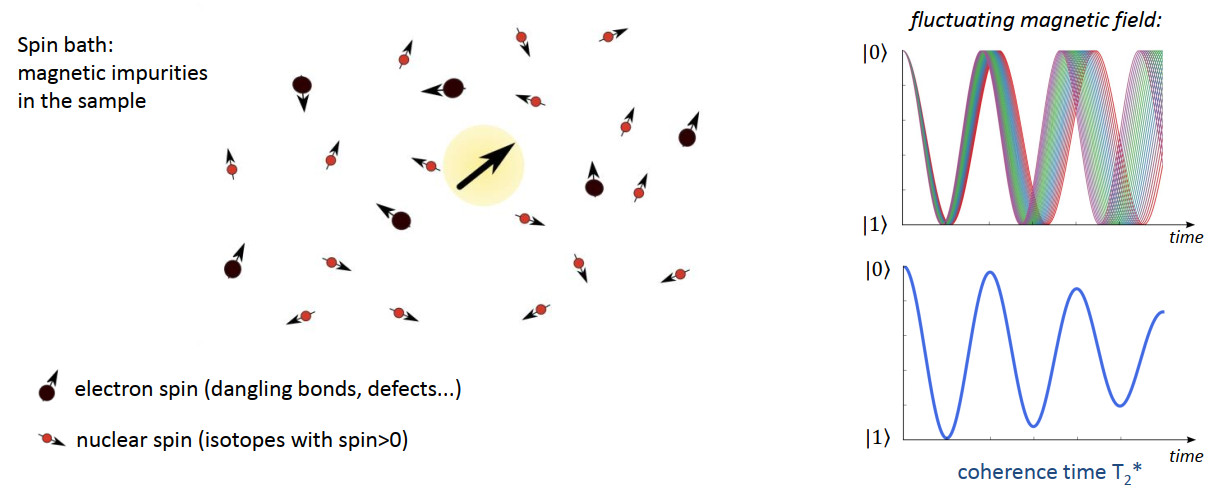
\includegraphics[width = 1\textwidth]{figures/T2_star.png}
\caption{On the left, the central electron spin is immersed in a "bath" given by other paramagnetic impurities and nuclear spins in the solid-state matrix. Given that the gyromagnetic ratio for electronic spins is $10^3-10^4$ larger than for nuclear spin, the priority in developing quantum-grade material is to eliminate paramagnetic impurities. On the right, the distribution in magnetic field given by the presence of different paramagnetic impurities and nuclear spins at different distances from the central spin results in a distribution of Larmor frequencies (top right). This leads to a decay of quantum coherence over time, characterised by a characteristic dephasing timescale $T_2^*$ (bottom right).}
\label{fig:T2_star}
\end{figure}

\subsection {Ramsey interferometry}
Let us consider a Stern Gerlach experiment, in two cases:
\begin{enumerate}
    \item an ensemble of $N$ spins, all prepared in the same quantum state $\ket{\psi} = \frac{1}{2} (\ket{\uparrow}+\ket{\downarrow})$. In this case there is a clear and well-defined phase relation ($\varphi = 0$) between $\ket{\uparrow}$ and $\ket{\downarrow}$ (the state can be written as $\ket{\psi} = \frac{1}{2} (\ket{\uparrow}+ e^{i \cdot 0}\ket{\downarrow})$). This state is a coherent superposition (pure state) described by the density matrix:
    \begin{equation}
        \rho = \frac{1}{2}\left(\begin{array}{cc}
1 & 1\\
1 & 1\end{array} \right)
    \end{equation}    
    \item an ensemble of $N$ spins, with $N/2$ in the state $\ket{\uparrow}$ and $N/2$ in the state $\ket{\downarrow}$. In this case there is no phase relation between $\ket{\uparrow}$ and $\ket{\downarrow}$, since the states belong to different particle. This is a mixed state described by the density matrix:
    \begin{equation}
        \rho = \frac{1}{2}\left(\begin{array}{cc}
1 & 0\\
0 & 1\end{array} \right)
    \end{equation}    
\end{enumerate}
In both cases, the Stern-Gerlach experiment will result in $50\%$ "spin-up" outcome, and $50\%$ "spin-down" outcome. So, the two states cannot be distinguished as such by spin measurements in the $\lbrace \ket{\uparrow}, \ket{\downarrow} \rbrace$.


Let us now apply a magnetic field $B$ along the $z$ direction. As we know, this results in a Zeeman splitting $\mathcal{E}_{\uparrow} = +\gamma \hbar B/2$ for $\ket{\uparrow}$ and $\mathcal{E}_{\downarrow} = -\gamma \hbar B/2$ for $\ket{\downarrow}$. Let us now consider what happens in the two cases.
\newline {\bf Pure state}. For the pure state, each of the two components pick up a phase, leading to $\ket{\psi} = \frac{1}{2} (e^{+i \gamma \hbar B t/2} \ket{\uparrow}+e^{-i \gamma \hbar B t/2} \ket{\downarrow})$, where $t$ is the time between the state is prepared and its measurement (known as {\bf free evolution time}). Collecting a (neglectable) global phase, the state can be written as:
\begin{equation}
\ket{\psi} = \frac{1}{2} ( \ket{\uparrow}+e^{-i \gamma \hbar B t} \ket{\downarrow})
\end{equation}. Again, the phase remains here well-defined, and equal to $\varphi = \gamma \hbar B t$. 
    \newline Suppose now to measure in a rotated basis, spanned by the orthogonal states $\lbrace \ket{+} = \frac{1}{2} ( \ket{\uparrow}+ \ket{\downarrow}), \ket{-} = \frac{1}{2} ( \ket{\uparrow}- \ket{\downarrow}) \rbrace$. The state can be written in this basis as:
    \begin{equation}
        \ket{\psi} = \frac{1}{2} \left [ \ket{+} + \ket{-} + e^{-i\varphi}\ket{+} - e^{-i\varphi}\ket{-} \right] = \ket{+} \left[ \frac{1 + e^{-i\varphi} }{2}\right] + \ket{-} \left[ \frac{1 - e^{-i\varphi} }{2}\right]
    \end{equation}
From this, the probability to detect the state $\ket{+}$ is:
\begin{equation}
    \mbox{Pr}(\ket{+}) = \mbox{cos}^2
\left( \gamma B t\right)
\end{equation}
From this equation, the probability to detect $\ket{+}$ oscillates between $0$ and $1$ as a function of the free evolution time $t$. This is a {\bf quantum interference} effect, originating from the coherence of the quantum state.
\newline {\bf Mixed state}. The situation is quite different for a mixed state. Now the state $\ket{\uparrow}$ picks up a phase $\varphi = +\gamma B t/2$, but it is just a global phase ($e^{i\gamma B t/2}\ket{\uparrow}$), not a relative phase between two states, and it can be neglected. Same thing happens to the $\ket{\downarrow}$ state: no phase relation is created between the two states. Therefore, when we measure them in the $\lbrace \ket{+}, \ket{-} \rbrace$ basis, we always get each outcome with $50\%$ probability, as we were getting in absence of magnetic field. There is no quantum interference here, and no oscillations: this state is {\bf incoherent}.

For quantum devices, we want the states to be coherent, since we want to exploit quantum coherence for practical applications (more about this later). However, in all practical cases, our qubits lose quantum coherence over time, changing from pure states to mixed states. In general, the outcome of the experiment we just described would be a series of oscillations that decay in amplitude as a function of the free evolution time $t$. The decay time is called {\bf dephasing time $T_2^*$}.

The experiment we just described is known as {\bf Ramsey experiment} and it can be used:
\begin{itemize}
    \item to measure an unknown magnetic field $B$, from the period of the coherent oscillations. Intuitively, the longer the oscillations last, the better we can measure their period (i.e. the better magnetic sensitivity we have)
    \item the measure the coherence time $T_2^*$, as the timescale over which the coherent oscillations decay
\end{itemize}
Typically, a Ramsey experiment is performed as follows:
\begin{enumerate}
\item the spin is initialised in $\ket{\uparrow}$
\item a $\pi/2$ pulse creates the equal superposition
\item the superposition is let to freely evolve under the magnetic field $B$ for a time $t$, picking up a relative phase as: 
\item a second $\pi/2$ pulse is applied to rotate the measurement basis (so we can measure in $\lbrace \ket{+}, \ket{-} \rbrace$, for example). Please note that one can include a control phase $\theta$ in this second $\pi/2$ pulse.
\item the spin is measured in the $\lbrace \ket{\uparrow}, \ket{\downarrow} \rbrace$. Again, the basis rotation has been performed in the previous step - this is exactly equivalent to measuring in a rotated optical polarisation basis by rotating a waveplate in front of a fixed polariser, if you are more familiar with optics.
\end{enumerate}
The probability to detect $\ket{\uparrow}$ goes as:
\begin{equation}
    \mbox{Pr}(\ket{\uparrow}) = e^{-(t/T_2^*)^2} \mbox{cos}^2
\left( \gamma B t + \theta\right)
\end{equation}
Note that here we have assumed a Gaussian decay of coherence with $T_2^*$: while this is pretty common in many real systems, it is not always the case and other decay laws can be found.

To conclude this pretty lengthy discussion, please note that a Ramsey experiment is mathematically equivalent to a Mach-Zender interferometer in optics.


\begin{table}[h]
\centering
\begin{tabular}{c | c }
configuration & hyperfine \\
\hline
$\ket{\Uparrow,  \Uparrow, \Uparrow}$ & $(A_1+A_2+A_3)/2$ \\
$\ket{\Uparrow,  \Uparrow, \Downarrow}$ & $(A_1+A_2-A_3)/2$ \\
$\ket{\Uparrow,  \Downarrow, \Uparrow}$ & $(A_1-A_2+A_3)/2$ \\
$\ket{\Downarrow,  \Uparrow, \Uparrow}$ & $(-A_1+A_2+A_3)/2$ \\
$\ket{\Downarrow,  \Downarrow, \Uparrow}$ & $(-A_1-A_2+A_3)/2$ \\
$\ket{\Uparrow, \Downarrow, \Downarrow}$ & $(A_1-A_2-A_3)/2$ \\
$\ket{\Downarrow,  \Uparrow, \Downarrow}$ & $(-A_1+A_2-A_3)/2$ \\
$\ket{\Downarrow,  \Downarrow, \Downarrow}$ & $(-A_1-A_2-A_3)/2$ \\
\end{tabular}
\caption{Example of distribution of $2^N$ hyperfine values for a bath of $N=3$ $I=1/2$ nuclear spins. We assume a hyperfine of the form $\mathcal{H}_I \sim A \hat{S}_z \hat{I}_z$.}
\label{tab:hyperfine}
\end{table}

\subsection {Spin baths and dephasing}
Why do quantum systems lose coherence and Ramsey fringes lose visibility? In the case of spin qubits, a major mechanism for the loss of quantum coherence ({\bf decoherence}) is the {\bf dephasing} associated to the bath of nearby impurities and nuclear spins in the material.
\newline Let's for the moment just consider nuclear spins, and let's assume our spin qubit is in silicon. Silicon is composed by three stable isotopes (see \href{https://en.wikipedia.org/wiki/Isotopes_of_silicon}{here}): $^{28}$Si and $^{30}$Si with nuclear spin $I=0$ and $^{29}$Si with $I=1/2$. $^{29}$Si contributes to around $4.4\%$ of the total concentration. This means that, around our central electron spin qubit, we have a diluted bath of $^{29}$Si nuclear spins ($^{28}$Si and $^{30}$Si do not possess a nuclear spin, so they do not contribute to the magnetic noise).
\newline Let us assume that the central electron spin just "feels" three $^{29}$Si nuclear spins. Since each of the $^{29}$Si $I=1/2$ spins has two possible configurations ($m_I=-1/2$: $\ket{\Downarrow}$ and $m_I=+1/2$: $\ket{\Uparrow}$), for three spins we have in total $2^3=8$ possible configurations of the bath ($\ket{\Uparrow, \Uparrow, \Uparrow}$, $\ket{\Uparrow, \Uparrow, \Downarrow}$, ..., $\ket{\Downarrow, \Downarrow, \Downarrow}$). Each of the three nuclear spins is coupled to the electron spin via a hyperfine interaction $\mathcal{H}_i \sim A_i \hat{S}_i \cdot \hat {I}_i$, resulting in the coupling strengths listed in Table \ref{tab:hyperfine}. 

Assuming that the electron spin is initially in a coherent superposition $\ket{\psi} = \frac{1}{\sqrt{2}} \left( \ket{\downarrow} + \ket{\uparrow} \right)$, each of the $8$ possible configurations of the bath result in $8$ possible evolutions of the electron spin, corresponding to 8 different Larmor frequencies for each electron spins state $\ket{m_s}$. As shown in Fig \ref{fig:T2_star}, the sum of sinusoids with slightly detuned frequencies leads to a decaying sinusoid, with the visibility of the fringes decaying over time. This is the physical origin of dephasing, and the decay time, in magnetic resonance terminology, is known as {\bf $T_2^*$ coherence time}. More formally, each of the $2^N$ possible evolutions ($8$, in this example) correspond to a wavefunction:
\begin{equation}
    \ket{\psi_i (\tau)} \propto \ket{\downarrow} + e^{i A_i \tau} \ket{\uparrow}
\end{equation}
In terms of density matrix, we would have:
\begin{equation}
\begin{split}
    \rho &= \sum p_i \ket{\psi_i} \bra{\psi_i}\\
    &= \sum p_i \left(\begin{array}{cc}
1 & e^{i A_i \tau} \\
e^{-i A_i \tau} & 1\end{array} \right)\\
    &= \left(\begin{array}{cc}
1 & \sum p_i e^{i A_i \tau} \\
\sum p_i e^{-i A_i \tau} & 1\end{array} \right)
\end{split}
\end{equation}

The off-diagonal elements of the density matrix resemble a Fourier series. Let's suppose we have many nuclear spins, described for simplicity by a Gaussian distribution of hyperfine values centred around zero and with variance $\sigma_A^2$:
\begin{equation}
    p_i = p(A_i) \propto e^{-A_i^2/(2 \sigma_A^2)}
\end{equation}
We can approximate the off-diagonal elements with a Fourier transform:
\begin{equation}
    \sum p_i e^{i A_i \tau} \sim \int e^{-A_i^2/(2 \sigma_A^2)} e^{i A_i \tau} dA_i \propto e^{-\sigma_A^2 \tau^2}
\end{equation}
This tells us that the off-diagonal elements of the density matrix decay to $0$ for longer $\tau$, with a Gaussian shape, leading to a mixed state. This happens on timescales on the order of $1/\sigma_A$, i.e. the wider the spread in the bath configurations, the faster the decay $T_2*$ to a mixed state (with off-diagonal elements to zero).

In general, a strategy to minimise dephasing and increase the spin coherence time $T_2^*$, as required by quantum applications, is to use materials that (mostly) feature isotopes with $I=0$ nuclear spin. As shown above for the case of silicon, one can find what stable isotopes an element X has, and which nuclear spins, on the Wikipedia page "Isotopes of X", for example.
 
\subsection {Hahn echo}
Can one restore quantum coherence once it has been lost due to dephasing?
\newline It turns out that this is actually possible, as long as one manages to "rephase" all the different oscillations that have gone out of phase. This concept was put forward by Erwin Hahn in 1950 and is now known as {\bf Hahn echo} or {\bf spin echo}.
\newline The idea is pretty simple. If you prepare a spin superposition at time $t=0$ and you let it evolve freely for a time $\tau$, it will pick up a set of phases $\varphi_I = \gamma_e B_i \tau$ depending on which magnetic field $B_i$ one considers, from the distribution of possible magnetic fields (as discussed above). At time $t = \tau$, one applies a $\pi$ pulse, inverting the spin, and letting it freely evolve again for a time $\tau$. Inverting the spin (i.e. swapping $\ket{\uparrow}$ with $\ket{\downarrow}$) is equivalent to inverting the phase evolution. In other words, the $\ket{\downarrow}$ component now picks a phase $\varphi_I = -\gamma_e B_i \tau$ up relative to the $\ket{\uparrow}$ component.
Therefore, at time $t=2\tau$ (i.e. with a dealy $\tau$ after the $\pi$ pulse), the two phases (one acquired in the time interval $[0, \tau]$, the other during time interval $[\tau, 2\tau]$) cancel out, and one recovers the initial state.
\newline If you want to picture this, you can think about a slow turtle and a fast dog running away from you, each at a different velocity $v_i$. Suppose they are trained to turn $180$ degrees at your whistle: if you whistle after a time $\tau$ and you wait a time $\tau$ after that (i.e. $2\tau$ in total) they will both be back to you, independently of how fast/slow each of them was going. Of course, this works as long as the process is static, i.e. they keep going at the same speed throughout the whole $2\tau$ interval.

Three important points:
\begin{itemize}
    \item the cancellation of the relative phase works no matter what the values of the possible $B_i$'s are, as long as they are static, i.e. they do not change over time. If the distribution of magnetic fields does change over time, then cancellation will not be perfect and coherence will decrease over time (more about this later)
    \item the cancellation of the relative phase works independently of the initial state. This means that any initial unknown state can be protected, with its coherence extended, which is very important for quantum memories.
    \item the protected coherent quantum states is not available at all points in time, but only at multiples of the echo time  $2\tau$. For a quantum memory, this means that an unknown quantum state stored in the memory can only  be accessed at multiples of $2\tau$.
\end{itemize}

\subsubsection{Echo time $T_2$}
Above, We briefly touched upon the idea that the different possible relative phases acquired by a spin superposition, corresponding to different possible magnetic fields, can be cancelled by a spin echo only only if the magnetic field distribution is static, i.e. it does not change over time.
\newline The magnetic field distribution, however, is not necessarily fixed over time. In the case of a nuclear spin bath, for example, interaction between the nuclear spin can lead to flip-flops, i.e. two nearby nuclear spins can swap their states. This changes the magnetic field $B_i$ acting on the electron spin, and the phases acquired before and after the $\pi$ pulse in the echo sequence do not cancel out perfectly.
\newline This leads to a decrease of spin coherence, which is known as {\bf echo time $T_2$}. This timescale characterises the decay of quantum coherence measured by a spin echo experiment.

A Hahn echo experiment is performed as follows:
\begin{enumerate}
\item the spin is initialised in $\ket{\uparrow}$
\item a $\pi/2$ pulse creates the equal superposition
\item the superposition is let to freely evolve under the magnetic field $B$ for a time $\tau$
\item a $\pi$ pulse is applied, to flip the spin state
\item a second $\pi/2$ pulse is applied to rotate the measurement basis (so we can measure in $\lbrace \ket{+}, \ket{-} \rbrace$, for example). Please note that one can include a control phase $\theta$ in this second $\pi/2$ pulse.
\item the spin is measured in the $\lbrace \ket{\uparrow}, \ket{\downarrow} \rbrace$. 
\end{enumerate}


\begin{figure}[h]
\centering
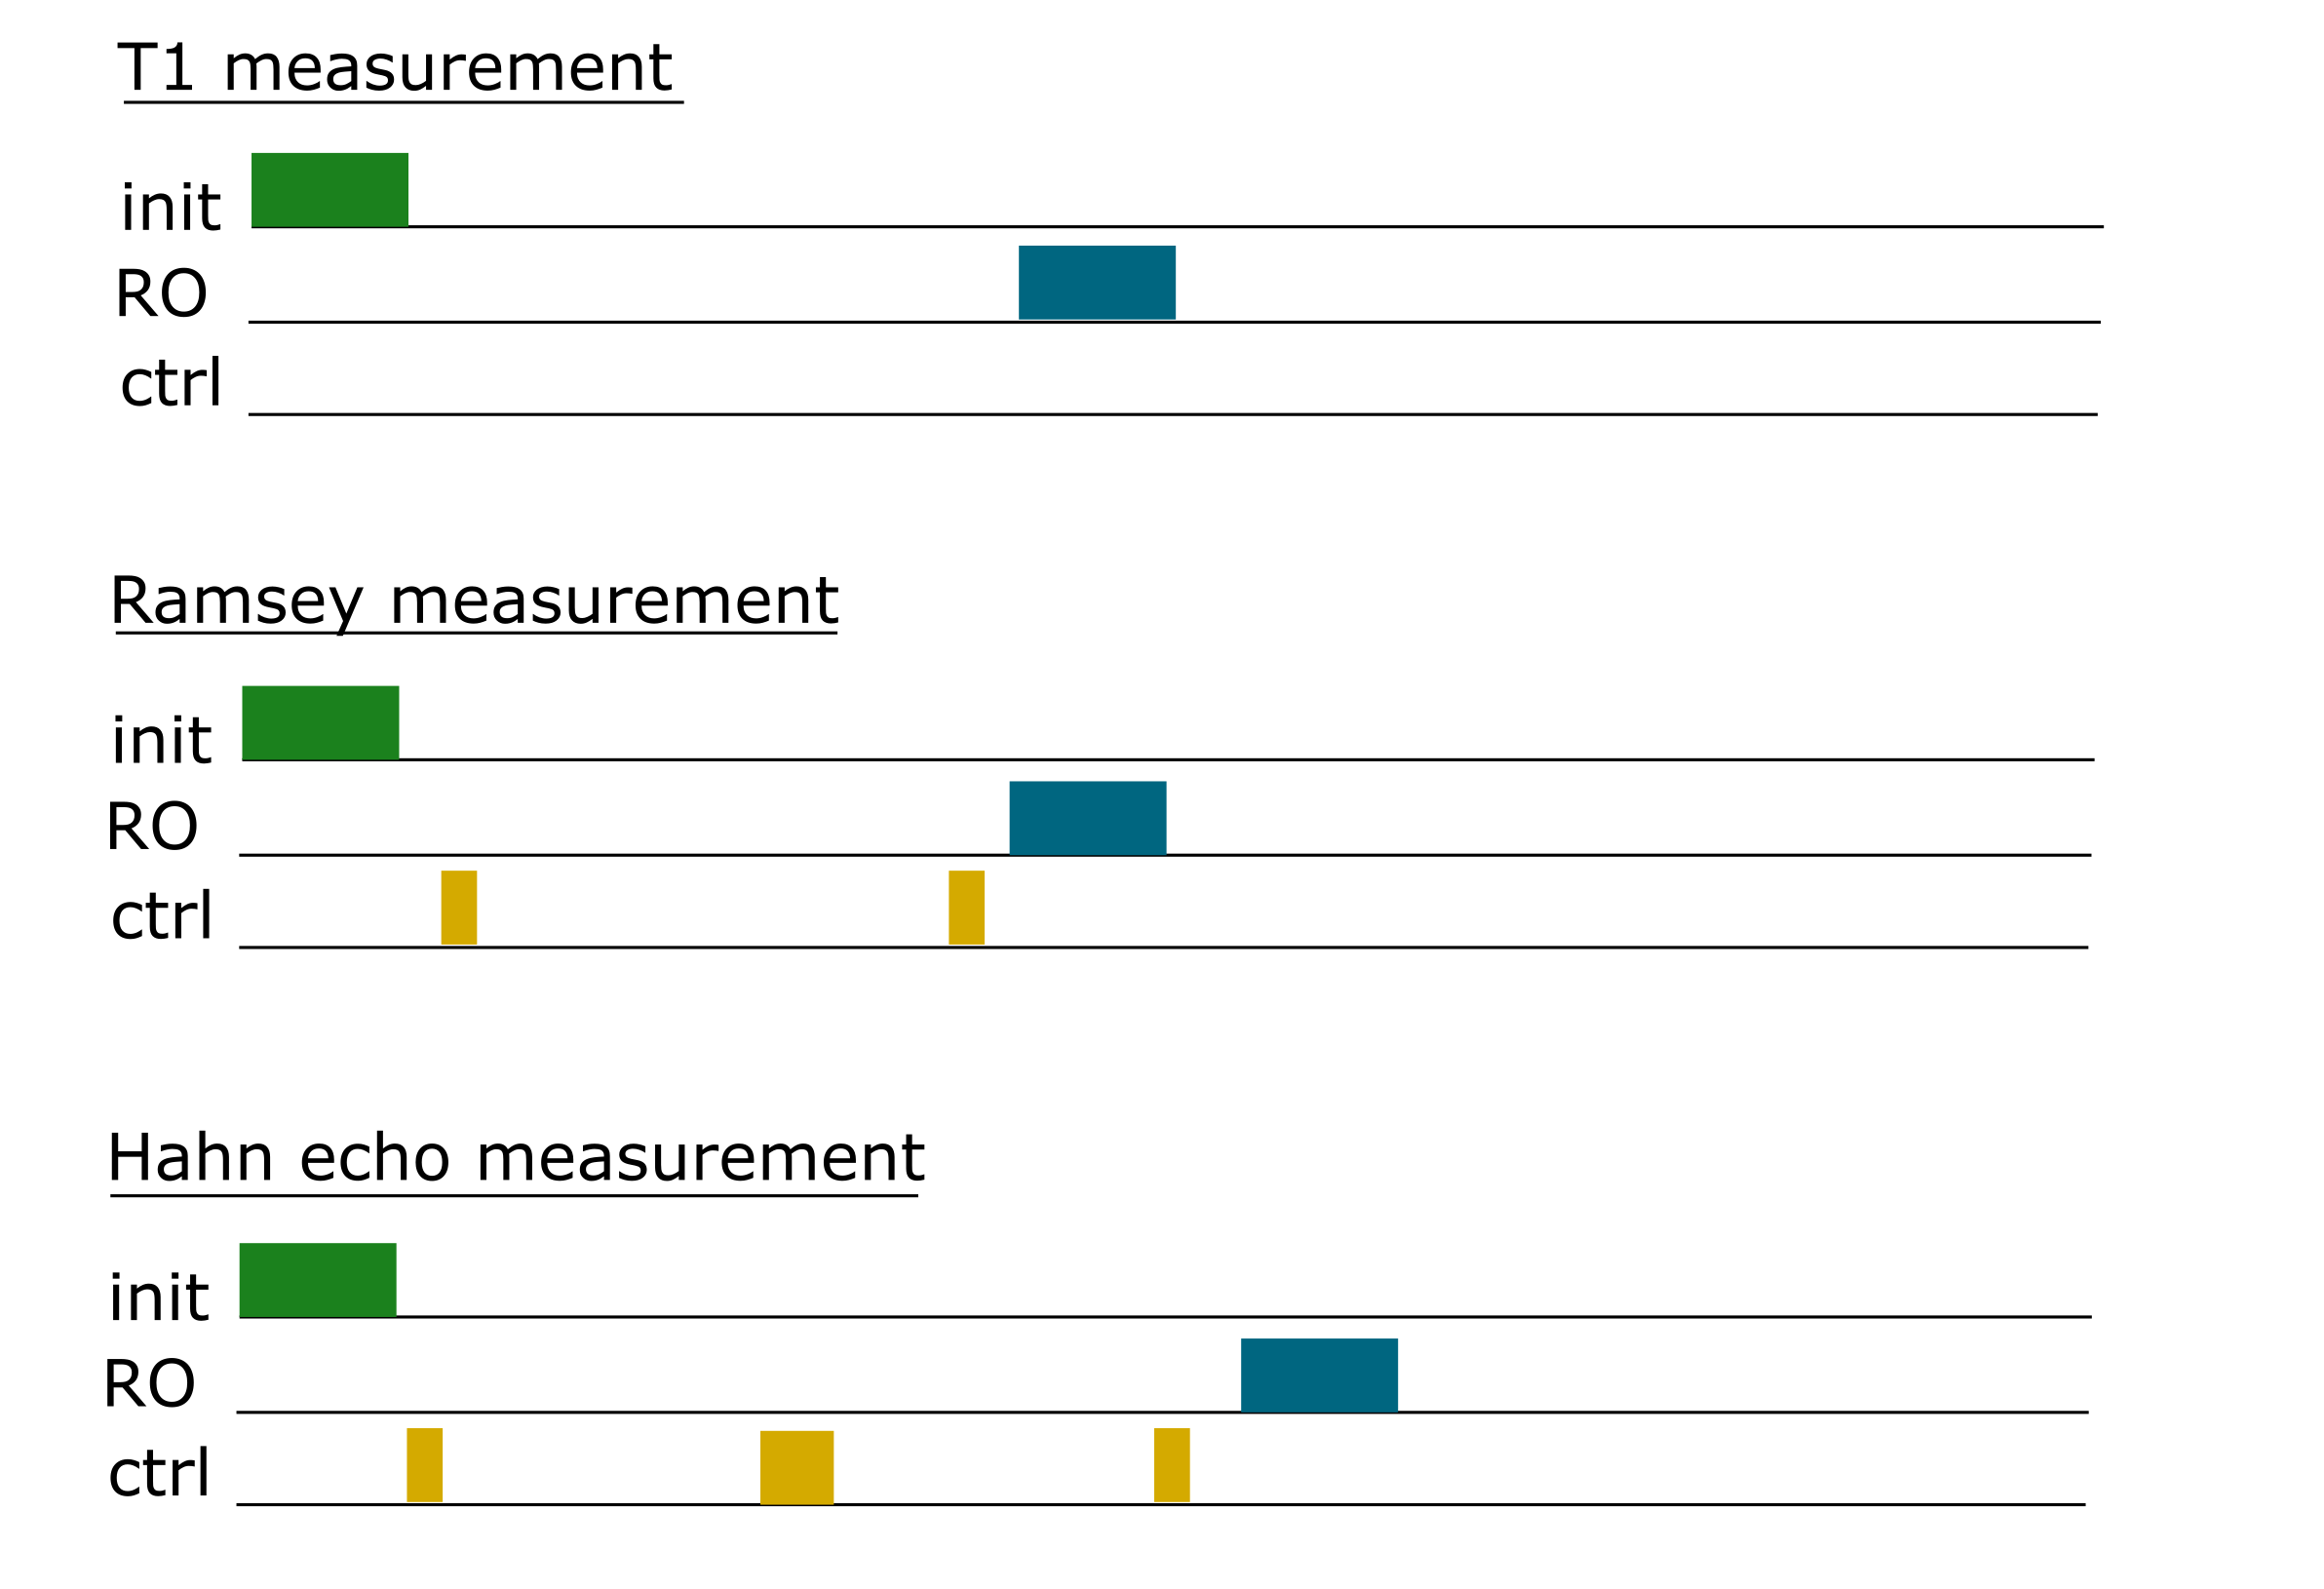
\includegraphics[width = 0.8\textwidth]{figures/pulse_sequence.png}
\caption{{\bf Summary of pulse sequences for standard experiments}. For each experiment, we outline when initialisation ("init"), readout ("RO") and control ("ctrl") pulses are activated. For the "control" line, the shorter pulses are $\pi/2$ pulses, the longer ones are $\pi$ pulses. }
\label{fig:pulse_sequences}
\end{figure}

\subsection {Summary of decoherence timescales}
We have discussed three different decoherence timescales:
\begin{itemize}
    \item the {\bf relaxation time $T_1$} (or spin-lattice relaxation) corresponds to the time it takes a polarised spin to decay into a thermal equilibrium state. At high temperature, this would correspond to the process:
    \begin{equation}
    \rho = \left(\begin{array}{cc}
        0 & 0\\
        0 & 1\end{array} \right) 
        \longrightarrow 
        \rho = \frac{1}{2} \left(\begin{array}{cc}
        1 & 0\\
        0 & 1\end{array} \right) 
    \end{equation}.
    At sufficiently low temperature and high magnetic field, such that the electron spin is thermally polarised into $\ket{\downarrow}$, the relaxation process corresponds to:
    \begin{equation}
    \rho = \left(\begin{array}{cc}
        0 & 0\\
        0 & 1\end{array} \right) 
        \longrightarrow 
        \rho =  \left(\begin{array}{cc}
        1 & 0\\
        0 & 0\end{array} \right) 
    \end{equation}.    
    The $T_1$ timescale can be measured by polarising the spin, for example in $\ket{\uparrow}$, and measuring its state as a function of time $t$. The probability for the spin to stay in the $\ket{\uparrow}$ state decays as $e^{-t/T_1}$.
    
    \item the {\bf dephasing time $T_2^*$} corresponds to the time it takes a coherent  spin superposition to decay into an incoherent mixture state described by the process:
    \begin{equation}
    \rho = \frac{1}{2}\left(\begin{array}{cc}
        1 & 1\\
        1 & 1\end{array} \right) 
        \longrightarrow 
        \rho = \frac{1}{2} \left(\begin{array}{cc}
        1 & 0\\
        0 & 1\end{array} \right) 
    \end{equation}.
    The $T_2^*$ timescale can be measured by a Ramsey experiment. Dephasing can be compensated by a spin echo experiment, as long as the distribution of magnetic fields is static.

    \item the {\bf spin echo time $T_2$} corresponds to the decay of coherence for a spin under a spin echo experiment. The $T_2^*$ timescale can be measured by a Hahn echo experiment and describes the timescales over which the magnetic field distribution is not static, for example due to flip-flops in the nuclear spin bath.
    
    \end{itemize}
    
\subsubsection{Example: NV centre in diamond}
If we consider, for example, the NV centre in diamond, $T_1$ is mainly determined by interaction with phonons through spin-orbit coupling. Diamond is a pretty stiff material, plus it's made of carbon, an element with small $Z$ (i.e. small spin-orbit coupling), leading to weak coupling to phonons. Therefore, $T_1$ times can be on the order of $10$ ms at room temperature, and several seconds at low temperature.

As we've seen, the $T_2^*$ time measured by a Ramsey experiment is determined by other paramagnetic impurities or nuclear spins in the diamond. Nowadays one can purchase very high-purity diamond grown by chemical vapour deposition, with very low concentration of paramagnetic impurities (mostly nitrogen, $<5$ parts per billion). Therefore $T_2^*$ is mostly limited by non-zero nuclear spins, which in diamond correspond to about $\sim 1.1\%$ of $^{13}$C nuclei with $I=1/2$ spin. This leads to $T_2^*$ on the order of a few microseconds. Techniques have been developed to grow {\bf isotopically purified} diamond, where the concentration of $^{13}$C nuclei is decreased to $\sim 0.01\%$:in this case $T_2^*$ can be extended to $100 \mu$s or so.
\newline Spin echo can be used to extend coherence time further, up to ms timescales. This limit depends on the flip-flop rates of nuclear spins in the bath.
\section{Quantum spintronic devices}
In this last section, we will go through a few example of different systems used in quantum spintronic devices, illustrating the operating principles of the device, and how spin control is performed.
\subsection {Example: NV centres at low temperature}
NV centres are naturally occurring defects in diamond, i.e. one can find NV centres in a diamond sample without creating them artificially. In case a higher concentration is needed, or to create them at specific positions, one can irradiate the sample with $^{14}$N or $^{15}$N ions and anneal the diamond to high temperature.

As discussed, NV centres are optically active, i.e. they emit photoluminescence when optically excite them. At low enough concentration, they can be isolated in a confocal microscope, exciting with a green laser and collecting photo-luminescence in the 600-800nm range. While the optical lifetime is $\sim 12$ns, i.e. one could expect up to $1/(12 \mbox{ns}) \sim 80 \cdot 10^6$ photons per second, typical photon fluxes are $\sim 40-100k$ counts per second. This is due to total internal reflection (which traps photons inside the diamond), optical losses in the microscope elements, and the finite detection efficiency of the single photon detectors. Optical collection efficiency can be improved by milling hemispherical solid immersion lenses on the diamond (the hemisheperes you can see in the SEM picture in Fig \ref{fig:NV_LT}(a), so that the photons come out always normal to the diamond surface, removing total internal reflection: this can increase the number of collected photons up to $1-1.5 \cdot 10^6$ counts per second.

When cooled to liquid helium temperatures ($T \sim 4$K), the NV centre displays narrow spin-dependent atomic-like optical transitions, that can be used for spin initialisation and readout (Fig. \ref{fig:NV_LT}(b)). Spin initialisation is performed by pumping the $A_1$ transition: while there is not a clear $\Lambda$-system, decay into $m_s = 0$ from the $m_s = \pm 1$ excited state is weakly allowed. For a long enough optical excitation, therefore, all population will be pumped into $m_s = 0$.

\begin{figure}[h]
\centering
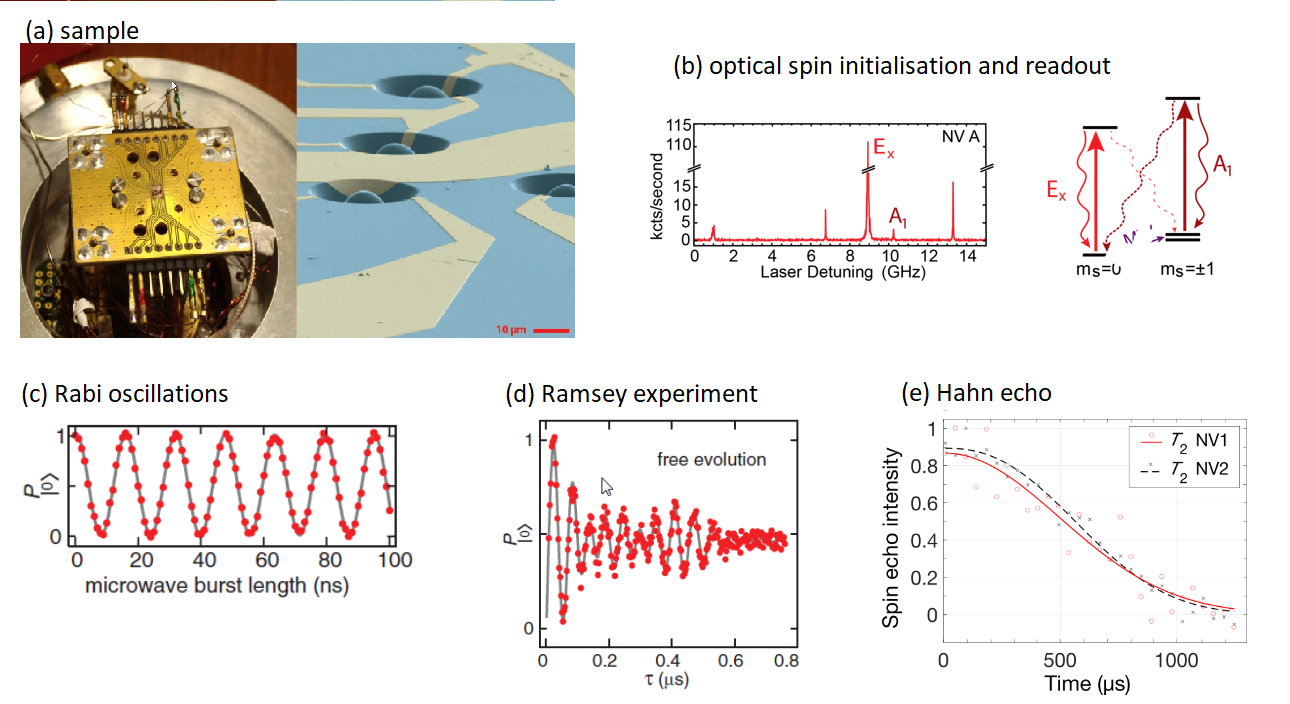
\includegraphics[width = 1\textwidth]{figures/NV_centre_LT.png}
\caption{{\bf Quantum spintronics with a single NV centre in diamond at low-temperature (from TU Delft)}. {\bf (a)} A sample holder with several ports for microwave delivery (including coplanar waveguides) and electrical DC contacts hosts a diamond sample (left). Solid immersion lenses are milled by focused ion beam to increase photon collection efficiency (by a factor $10$x-$20x$ (right). {\bf (a)} High-fidelity single-shot electron spin initialisation and readout is performed by optical excitation of narrow spin-selective transitions within the defect zero-phonon line (from \cite{robledo_high-fidelity_2011}). The $E_x$ transition is a "cycling" transition that couples to $m_s=0$, generating a sufficient number of photon to discriminate the spin state, when excited. The $A_1$ transition is a "spin-flip" transitions that couples to $m_s = \pm 1$ and, when excited, eventually decays into $m_s = 0$, enabling polarisation into $m_s = 0$. The transitions $E_x$ and $A_1$ can be differentiated, and selectively excited, because they appear at slightly different frequencies (about $1$ GHz apart). {\bf (c)} High-fidelity Rabi oscillations between $m_s = 0$ and $m_s = -1$, achieved by driving microwave pulses of different lengths resonant with the $m_s = 0 \leftrightarrow -1$ ground-state spin transition. {\bf (d)} Ramsey experiment, showing $T_2^* \sim 0.6 \mu$s. {\bf (e)} Hahn echo experiment, showing $T_2 \sim 0.7$ ms.}
\label{fig:NV_LT}
\end{figure}

Spin detection is performed by exciting the $E_x$ transition (which selectively couples to $m_s = 0$). This is a so-called "cycling" transition, that does only have a really small decay rate into $m_s = \pm 1$ (therefore maximising the number of time we "cycle" between ground and excited state emitting photons). If the spin state is $m_s = 0$, then we will get photons out, otherwise we will not. If optical collection is high enough, we can collect enough photons to determine the spin photons before eventually flipping into $m_s = \pm 1$, enabling single-shot readout. Experiments on samples with solid immersion lenses have shown single-shot electron spin readout with fidelities as high as $96\%$ for $m_s = 0$ and $99\%$ for $m_s = 1$.

Spin control is performed by microwaves delivered to the sample through an antenna, for example an on-chip stripline in Fig \ref{fig:NV_LT}. The NV centre features a so-called zero-field splitting (essentially an effective built-in magnetic field originating from the breaking of rotational symmetry created by the crystal lattice) of 2.8 GHz: even at small magnetic fields, one needs to apply the microwaves around 3 GHz. An example of Rabi oscillations can be found in Fig \ref{fig:NV_LT}, together with Ramsey and Hahn echo experimental data. The fringes in the Ramsey experiment are due to the magnetic field induced by the $^{14}$N nuclear spin ($I=1$) associates with the NV's own nitrogen atom (which couples to the electron spin with a hyperfine $A \sim 2.18$ MHz.

The nitrogen nuclear spin can also be used an additional qubit (as potentially $^{13}$C nuclear spins in the bath). As discussed, nuclear spins have gyromagnetic ratio much smaller (a factor $10^3-10^4$) then electron spins: since they couple much less to magnetic noise, they feature much longer coherence times (e.g. $T_2^* \sim 10$ ms). Therefore, nuclear spins are quite useful as quantum memories.

\subsection {Example: $^{31}$P donor in silicon}
Semiconductors provide a natural mechanism for trapping single spins: using electrons bound to individual donor atoms at low temperature. A donor atom is a dopant with one additional electron, for example phosphorus. To incorporate donor-based spins into nanoscale devices, it is necessary to position electrostatic gates with respect to the donor and to position many donors with respect to each other (the precision that is required depends on the precise architecture that is sought).

As for NV centres, donor atoms can be positioned in silicon by using ion implantation, even at the level of individual donors, although the precision with which this can be achieved is limited to approximately 10 nm. Transport measurements — in which electrons tunnel through individual implanted donor atoms in metal–oxide–semiconductor field-effect transistor (MOSFET)-like devices — can be performed. Recently, it was shown that donors can be tunnel-coupled directly to silicon single-electron transistors, an architecture that allows measurement with a large signal-to-noise ratio. Moreover, donors can be positioned with extremely high precision by using a lithographic technique based on the removal of a hydrogen resist by a scanning tunnelling microscopy tip. Lines of donors for use as leads and gates can also be fabricated in this way, allowing the precise alignment of a cluster of a few donors or a single donor.

As we have seen, the spin of the dopant electron can be measured by spin-selective tunneling. A strong magnetic field splits the $\ket{\downarrow}$ and $\ket{\uparrow}$ states, so that the higher-energy state has sufficient energy to tunnerl out. By having the electron tunnel from the donor onto the island of a nearby single electron transistor (SET), one can detect the tunneling event, inferring the initial spin state. Spin control is typically achieved by driving microwaves with an on-chip stripline very close to the dopant.

For the interested reader, more information about these systems can be found in  \cite{morton_embracing_2011} and \cite{zwanenburg_silicon_2013}.

\subsection {Example: electrostatic quantum dot}
A quantum dot is an artificially structured system that can be filled with electrons or holes. The dot can be coupled via tunnel barriers to reservoirs, with which electrons can be exchanged. By attaching current and voltage probes to these reservoirs, one can measure its electronic properties. The dot is also coupled capacitively to one or more gate electrodes, which can be used to tune the electrostatic potential of the dot with respect to the reservoirs.
\newline The electronic properties of quantum dots are dominated by two effects. First, the Coulomb repulsion between electrons on the dot leads to an energy cost for adding an extra electron to the dot. Due to this charging energy tunneling of electrons to or from the reservoirs can be suppressed at low temperatures (Coulomb blockade, as you have seen in part-A of this course). Second, the confinement in all three directions leads to quantum effects that influence the electron dynamics. Due to the resulting discrete energy spectrum, quantum dots behave in many ways as artificial atom.

Historically, the main system widely used in labs working on quantum devices have been lateral GaAs quantum dots. These are fabricated from heterostructures of GaAs and AlGaAs grown by molecular beam epitaxy. By doping the AlGaAs layer with Si, free electrons are introduced. These accumulate at the GaAs/AlGaAs interface, typically 50-100 nm below the surface, forming a two-dimensional electron gas (2DEG) - a thin ($\sim 10$ nm) sheet of electrons that can only move along the interface. The 2DEG can have high mobility and relatively low electron density (typically $10^5 - 10^7$ cm$^2$/V s and $\sim 1-5 \cdot 10^15 m^{-2}$, respectively. The low electron-density results in a large Fermi wavelength $\sim 40$ nm and a large screening length, which allows us to locally deplete the 2DEG with an electric field. This electric field is created by applying negative voltages to metal gate electrodes on top of the heterostructure.
Electron-beam lithography enables fabrication of gate structures with dimensions down to a few tens of nanometers, yielding local control over the depletion of the 2DEG with roughly the same spatial resolution. Small islands of electrons can be isolated from the rest of the 2DEG by choosing a suitable design of the gate structure, thus creating quantum dots. Finally, low resistance (Ohmic) contacts are made to the 2DEG reservoirs. To access the quantum phenomena in GaAs gated quantum dots, they have to be cooled down to well below 1 K (typically in dilution refrigerators with base temperatures of $\sim 20$ mK).

Electron spin initialisation and readout is performed by spin-selective tunneling in a quantum dot coupled to a charge sensor (such as a quantum point contact). Spin manipulation is achieved by microwave driving, by an on-chip stripline.

In the last few years, research labs have been able to demonstrate spin control in silicon quantum dots. This is a crucial technological achievement, since silicon features a much lower concentration of nuclear spins (and thereby a much longer electron spin coherence time) and it is of course extremely advantageous due to its full compatibility with standard CMOS industrial nano-fabrication processes.

For the interested reader, more information about these systems can be found in \cite{hanson_spins_2007}, \cite{morton_embracing_2011} and \cite{zwanenburg_silicon_2013}.


\subsection {Applications to quantum sensing}
A single spin is the smallest possible magnetic spin sensor, capable of detecting magnetic fields (through the Zeeman splitting) with nanoscale spatial resolution. Most spin-based sensing experiments are performed by exploiting the NV centre in diamond, due to the capability to polarise and detect its spin state even at room temperature.

\begin{figure}[h]
\centering
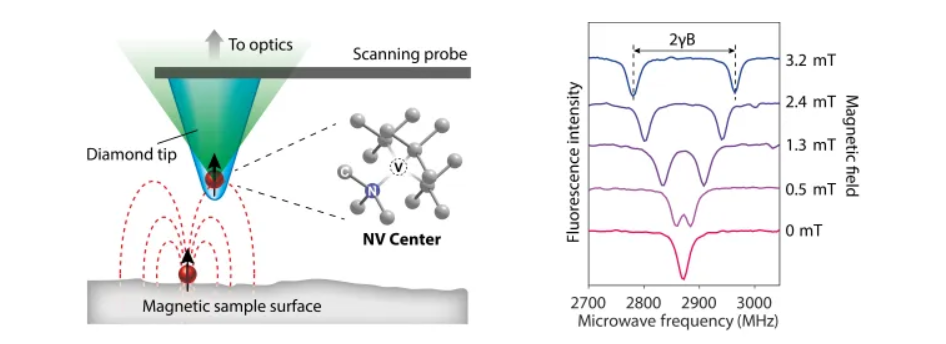
\includegraphics[width = 1\textwidth]{figures/ODMR_sensing.png}
\caption{{\bf Quantum sensing with a single NV centre in diamond (from QZabre)}. On the left, sketch of a quantum sensing experiment with a single electronic spin associated to a nitrogen-vacancy centre in diamond on a diamond AFM tip. The diamond tip is scanned over a sample and allows retrieving a map of magnetisation with nanoscale spatial resolution. On the right, the magnetic field is measured by collecting photo-luminescence under green laser excitation as a function of the microwave drive frequency. When the microwave frequency is resonant with the $m_s = 0 \leftrightarrow m_s = -1$ or $m_s = 0 \leftrightarrow m_s = +1$ transition, the photoluminescence decreases, exhibiting a dip. The frequency of the dip, related the Zeeman shift, allows to measure the magnetic field projection along the NV axis.}
\label{fig:ODMR_sensing}
\end{figure}


We have seen in Section that resonant optical excitation at low temperature can achive high-fidelity initialisation and single-shot readout of single electronic spins associated with NV centres in diamond. However, the outstanding property that makes NV centres so interesting is that there spin state can be detected even at room temperature, albeit with reduced contrast (no single-shot, only averaged readout). This can be performed by simply illuminating the NV with a green laser for $\sim 1 \mu$s. Typically $\sim 0.03$ photons/shot are detected when the electron spin is in $m_s=0$ and $\sim 0.02$ photons/shot for the electron in $m_s=1$. These values clearly do not allow spin state discrimination in a single shot (most of the times one gets just no photons out), but when averaging over several repetitions enough statistics is accumulated. For example, averaging over $100,000$ repetitions one would get $2,000$ photons for $m_s=1$ and $3,000$ for $m_s=0$, which can be comfortably distinguished above the shot noise limit.
\newline The reason single-shot readout cannot be achieved is that after $\sim 1\mu$s the spin is pumped into $m_s=0$, destroying all spin information before one can get a statistically significant number of photons out.

Several research groups have shown that NV centres can be integrated in diamond AFM tips, which can be scanned across samples to measure magnetisation with spatial resolution of $20-30$ nm.
\newline Alternatively, research groups have been using NV centres in small nanodiamonds (few tens of nanometer in size). Diamond is a quite inert material, and fully bio-compatible: nano-diamond with NVs have been introduced in cell to monitor physical quantities inside the cell with nanoscale spatial resolution.

In the following, we will examine a couple of different sensing situations.

\subsubsection{DC sensing}
As we have seen, a static (DC) magnetic field modifies the energy levels through the Zeeman shift, shifting also the frequency of the transitions between $m_s = 0$ and $m_s = \pm 1$. By monitoring the frequencies of the transitions through optically-detected magnetic resonance (ODMR), one can map the static magnetic field at each position.

\subsubsection{Relaxometry}
In this case, the quantity of interest is not a magnetic signal, but noise. We have seen that the main mechanism for $T_1$ relaxation is coupling to phonons, but coupling to a large number of paramagnetic impurities (unpaired electrons) can also decrease the $T_1$ lifetime. In a biological environment, for example, radicals feature unpaired electrons which can decrease $T_1$. Since radicals are, for example, associated with stress, the capability to monitor radicals with nanoscale resolution inside a living cell is quite important.

\subsection {Applications to quantum computing}
Quantum computers are machines that exploit quantum superposition and entanglement in qubits to provide faster computations for certain classes of problems.
\newline There is much research going on in developing a fully-working fault-tolerant quantum computer, based on different materials/devices platforms. Recently, Google demonstrate full coherent control of $53$ qubits based on superconducting circuits (more about this next week). Spins in silicon are also good candidates for quantum computing, due to their long $T_1$ at temperatures around $1$K (in contrast to superconducting qubits that require complex operation at mK temperatures) and the established processing for the silicon platform.

%Here, we will briefly discuss an example about how spin-based quantum gates are implemented and we will then look into a couple of specific architectures.

\begin{comment}
\subsubsection{Example: electron-nuclear quantum gates}
Consider a $S=1/2$ electronic spin coupled to a $I=1/2$ nuclear spin. We assume the hyperfine interaction has the form:
\begin{equation}
    \mathcal{H}_I \sim A S_z I_z
\end{equation}
We label the electron spin states by $\lbrace \ket{\uparrow} = \ket{m_s=+1/2}, \ket{\downarrow}= \ket{m_s=-1/2} \rbrace$ and the nuclear spin states by $\lbrace \ket{\Uparrow}= \ket{m_I=+1/2}, \ket{\Downarrow}= \ket{m_I=-1/2} \rbrace$.
\newline Suppose to prepare at $t=0$ both electron and nuclear spins in equal superpositions. The joint (product) state is:
\begin{equation}
    \ket{\psi} = \frac{1}{2} \left[ \ket{\uparrow, \Uparrow} + \ket{\uparrow, \Downarrow} + \ket{\downarrow, \Uparrow} + \ket{\downarrow, \Downarrow} \right]
\end{equation}
If we let this state freely evolve for a time $\tau$ under the Hamiltonian $\mathcal{H}_I$, we get:
\begin{equation}
    \ket{\psi} = \frac{1}{2} \left[ e^{iAt/4} \ket{\uparrow, \Uparrow} + e^{-iAt/4} \ket{\uparrow, \Downarrow} + e^{-iAt/4} \ket{\downarrow, \Uparrow} + e^{+iAt/4} \ket{\downarrow, \Downarrow} \right]
\end{equation}
Collecting $e^{+iAt/4}$ and neglecting global phases:
\begin{equation}
    \ket{\psi} = \frac{1}{2} \left[ \ket{\uparrow, \Uparrow} + e^{-iAt/2} \ket{\uparrow, \Downarrow} + e^{-iAt/2} \ket{\downarrow, \Uparrow} + \ket{\downarrow, \Downarrow} \right]
\end{equation}

\end{comment}



\begin{figure}[h]
\centering
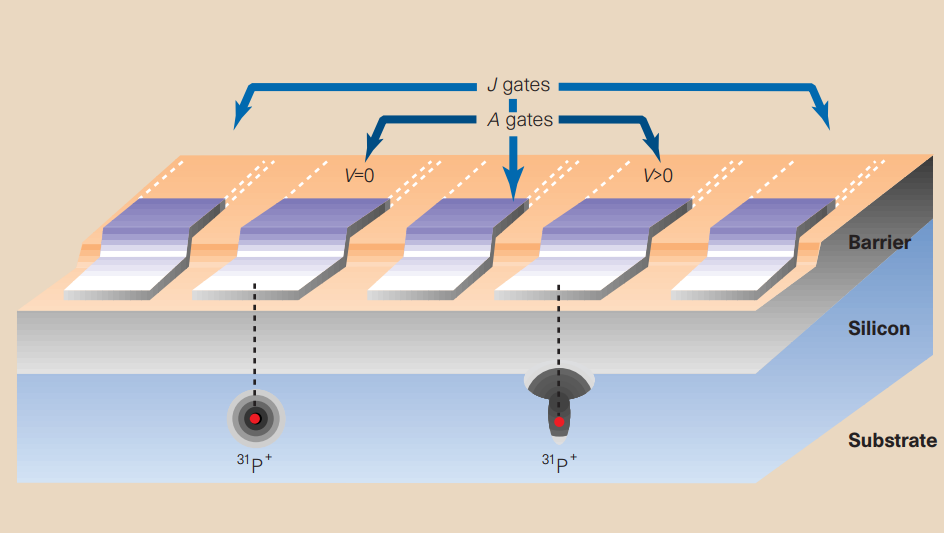
\includegraphics[width = 0.8\textwidth]{figures/kane_QC.png}
\caption{Kane's quantum computer proposal, based on coupled electronic and nuclear spins associated to $^{31}$P donors in Si. Coupling between neighbouring electronic spins is achieved by the exchange coupling, controlled by `$J$' electrodes which change the overlap between electron wavefunctions.}
\label{fig:kane}
\end{figure}

\subsubsection{Kane's proposal for a quantum computer}
The proposal elaborated by Kane (\cite{kane_silicon-based_1998}) is based on phosphorus ($^{31}$P) donor impurities in silicon placed in an array with a spacing of $\sim 20$ nm, approximately $20$ nm below the surface. An insulating SiO$_2$ layer is grown on top of the silicon, with metal gates deposited on the oxide above each donor (A gates), and between adjacent donors (J gates).
\newline The silicon substrate is isotopically-purified $^{28}$Si, will all Si atoms feature nuclear spin $I = 0$. Qubits are implemented Using the $I=1/2$ nuclear spin of the $^{31}$P donors. As we have seen, nuclear spins have very long coherence times and can be controlled by radio-frequency pulses in the MHz range. 
By altering the voltage on the A gates, it should be possible to alter the Larmor frequency of individual donors. This allows them to be addressed individually, by bringing specific donors into resonance with the applied oscillating magnetic field.


Due to their small gyromagnetic ration, nuclear spins do not interact significantly with each other unless they are $<1$nm apart. In the Kane configuration, with nuclear spins 20 nm away, there is no way to exploit the interaction between the nuclear spins to create quantum gates. This can be done by exploiting the electron spin in the donor. The quantum state encoded on the nuclear spin is transferred from the nucleus to the donor electron. Then, a potential is applied to the J gate, drawing adjacent donor electrons into a common region, greatly enhancing the interaction between the neighbouring spins. By controlling the J gate voltage, two-qubit operations are possible.

Kane's proposal for readout was to apply an electric field to encourage spin-dependent tunneling of an electron to transform two neutral donors to a D+–D– state, that is, one where two electrons orbit the same donor. The charge excess is then detected using a single-electron transistor. This method has two major difficulties. Firstly, the D– state has strong coupling with the environment and hence a short decoherence time. Secondly and perhaps more importantly, it's not clear that the D– state has a sufficiently long lifetime to allow for readout—the electron tunnels into the conduction band. 

\section {Appendix}
{\bf This section is optional} and not part of the assessment. It is only for students interested about how spin is justified within relativistic quantum mechanics. These notes were kindly provided by Leone di Mauro Villari.

\subsection{Derivation of the Dirac equation}
\label{sec:dirac}
The Dirac equation is a relativistic wave equation derived in 1928 by British physicist Paul Dirac \cite{DiracP}. It describes massive spin-$\frac{1}2$ particles and it was proposed to solve the problem of the negative energy solutions of the Klein-Gordon equation. At that time antimatter was yet to be discovered and there were no physical explanations for negative energy solutions. Dirac postulated a first order wave equation of the form 
\beq \label{Dirac1}
i \hbar \frac{\partial}{\partial t} \psi = ( c \boldsymbol{\alpha} \cdot \mathbf{p} + m c^2 \beta ) \psi,
\eeq
where $\p=- i \hbar \nabla$ is the momentum operator.  This is in fact a different way of writing the square root in the Schr\"odinger equation for a relativistic particle 
\beq  \label{Dirac2}
i \hbar \frac{\partial}{\partial t} \psi = \sqrt{p^2c^2 + m^2 c^4} \psi,
\eeq
that contains an ill-defined pseudo-differential operator. This means that the Dirac first quantised Hamiltonian $H =  c \boldsymbol{\alpha} \cdot \mathbf{p} + m c^2 \beta $ has to satisfy the following relation 
\beq  \label{Dirac3}
  (m c^2 \beta + c \boldsymbol{\alpha} \cdot \mathbf{p}) ^2 =  p^2c^2 + m^2 c^4, 
\eeq
to ensure consistency with both quantum mechanics (Schr\"odinger equation) and special relativity. Equation (\ref{Dirac3}) poses constraints on the coefficients $\boldsymbol \alpha$ and $\beta$. Expanding the square we get the following conditions 
\beq \label{cliff}
\{\beta, \alpha_i\} = 0, \quad \beta^2 = I, \quad \alpha_i^2 = I,
\eeq
where $\{\cdot \}$ is the anti-commutator, $i = (1,2,3)$ and $I$ the identity matrix. Relations \ref{cliff} tells us that $\boldsymbol \alpha$ and $\beta$ have to be square matrices with zero trace.  This means that the dimension of the vector space to which they belong must be even \cite{bd}. In $M_2(\mathbb{C})$, the space of $2 \times 2$ complex matrices there are only three independent matrix that satisfy the Clifford algebra in equations (\ref{cliff}), the Pauli matrices. This is not a viable choice as we need four matrices ($\alpha_i,\beta$), we find them in the $M_4(\mathbb{C})$ vector space and they are written as 
\beq
\beta = \left(\begin{array}{cc}I_2 & 0 \\0 & -I_2\end{array}\right) \quad \alpha_i = \left(\begin{array}{cc}0& \sigma_i \\ \sigma_i & 0\end{array}\right),
\eeq
where $I_2$ is the $2 \times 2$ identity matrix and $\sigma_i$ the Pauli matrices. Multiplying both sides of equation (\ref{Dirac1}) by $\beta$ and defining the Dirac matrices 
\beq
\gamma_0 = \beta, \quad \gamma_i = \beta \alpha_i,
\eeq
we can write the Dirac equation in the conventional form
\beq \label{Dirac4}
i \hbar \gamma^\mu \partial_\mu \psi - m c^2 \psi = 0,
\eeq
where $\mu = (0,1,2,3)$. 

The solution of the Dirac equation is doubly degenerate, in particular there are two solutions (spin up and spin down) with positive energy and two with negative energy. Linearising the square root in equation (\ref{Dirac2}) does not eliminate the negative energy eigenstates. This was a big theoretical step towards the discovery of antimatter as it was the first solid evidence that negative energy excitations were physically meaningful. It led Dirac to the formulation of the Hole theory that describes the vacuum as the quantum state in which all the negative-energy electron eigenstates are occupied \cite{DiracP}. \\Positive and negative energy eigenstates are found relatively easily in momentum space as the following four-spinors 
\beq
\vec u^{\,(\sigma)}_{\p} = \sqrt{\frac{E_\p + m \,c^2}{2m\,c^2}}\left(\begin{array}{c}\varphi^{(\sigma)} \\ \frac{ \boldsymbol{\sigma} \cdot \mathbf p \,c}{E_\p + m\,c^2} \varphi^{(\sigma)} \end{array}\right), \quad \quad
\vec v^{\,(\sigma)}_{\p} = \sqrt{\frac{E_\p + m\,c^2}{2m\,c^2}}\left(\begin{array}{c}  \frac{ \boldsymbol{\sigma} \cdot \mathbf p\, c}{E_\p + m\,c^2} \chi^{(\sigma)}  \\ \chi^{(\sigma)} \end{array}\right),
\eeq
where $\sigma=(\uparrow,\downarrow)$ is the spin-projection quantum number, $\varphi^{(\sigma)}$ and $\chi^{(\sigma)}$ are two-spinors and $E_\p = \sqrt{p^2c^2 + m^2c^4}$. The general, quantised, spinor solution of equation (\ref{Dirac4}) can be written in terms of the eigenstates as 
\beq
\vec \psi(\rr,t) = \sum_{\sigma=1}^2 \int d\p \,  \sqrt{\frac{m c^2}{2 \pi^3 E_\p}} (\hat a_\p^{(\sigma)}  \vec u^{\,(\sigma)}_{\p}  e^{i(\kk \cdot \rr - \omega_\p t) }+ \hat b^{(\sigma) \, \dagger}_\p \vec v^{\,(\sigma)}_{\p}  e^{-i(\kk \cdot \rr - \omega_\p t)}),
\eeq
where $\hat a_\p^{(\sigma)}$, ($\hat b_\p^{(\sigma)}$) are electron, (positron) annihilation operators satisfying the following anti-commutation relations 
\beq
\{\hat a_\p^{(\sigma)},\hat a^{(\sigma)\, \dagger}_{\p'}\} = \{\hat b_\p^{(\sigma)}, \hat b^{(\sigma) \, \dagger}_{\p'}\} = \delta_{\sigma,\sigma'} \delta(\p-\p').
\eeq

\subsection{Non-relativistic limit}
\label{sec:dirac_spin}
The main topic of this thesis are systems with a pseudo-relativistic dispersion relations in condensed matter physics. Hence, it is important to study how to connect the relativistic physics of the Dirac equation with the non-relativistic physics of condensed matter systems. In other words we will compute the non-relativistic limit of the Dirac equation. To do so we start from equation (\ref{Dirac1}) and we add an external four vector potential $A_\mu=(\mathbf{A},\Phi)$ with the minimal coupling in Gaussian units 
\beq 
\mathbf{p} \to \boldsymbol{\pi} = \p - \frac{e}c \A, \quad \quad H \to H + e \Phi, 
\eeq
where $e$ is the electron charge and $c$ the speed of light. The Dirac equation thus becomes 
\beq \label{Dirac5}
i\hbar \frac{\partial}{\partial t} \vec \psi = ( c\, \boldsymbol{\alpha} \cdot \boldsymbol \pi +  \beta mc^2 + e \Phi)\vec \psi.
\eeq
It is convenient to work in the bi-spinor representation \footnote{A bi-spinor is an element of a four dimensional complex vector space considered as a $(\tfrac{1}2,0)\oplus(0,\tfrac{1}2)$ representation of the Lorentz group.}
\beq
\vec \psi = \left(\begin{array}{c}\tilde\varphi \\\tilde \chi\end{array}\right)
\eeq
and write equation (\ref{Dirac5}) as
\beq  \label{Dirac6}
i \hbar  \frac{\partial}{\partial t}  \left(\begin{array}{c}\tilde\varphi \\\tilde \chi\end{array}\right) = c\, \boldsymbol \sigma \cdot \boldsymbol \pi  \left(\begin{array}{c}\tilde\chi \\\tilde \varphi \end{array}\right) + mc^2  \left(\begin{array}{c}\tilde\varphi \\ -\tilde \chi\end{array}\right) + e\Phi  \left(\begin{array}{c}\tilde\varphi \\\tilde \chi\end{array}\right).
\eeq
In the non relativistic limit $v/c \ll 1$ the rest energy $m c^2$ is the largest energy scale, thus we can parametrise the spinor as follows
\beq
\left(\begin{array}{c}\tilde\varphi \\\tilde \chi\end{array}\right) = e^{i\frac{mc^2}\hbar t} \left(\begin{array}{c}\varphi \\  \chi\end{array}\right)
\eeq
where $\varphi$ and $\chi$ are slowly varying functions of time and are solutions of 
\beq  \label{Dirac7}
i \hbar  \frac{\partial}{\partial t}  \left(\begin{array}{c}\varphi \\  \chi\end{array}\right) = c\, \boldsymbol \sigma \cdot \boldsymbol \pi  \left(\begin{array}{c}\chi \\  \varphi \end{array}\right) -2 mc^2 \left(\begin{array}{c}0 \\  \chi\end{array}\right) + e \Phi \left(\begin{array}{c}\varphi \\  \chi\end{array}\right),
\eeq
assuming that the scalar potential field $e \Phi$ and the kinetic energy are both much smaller than the rest mass the second of equations (\ref{Dirac7}) is solved as
\beq \label{chi}
\chi = \frac{\boldsymbol \sigma \cdot \boldsymbol \pi}{2mc},
\eeq
this equation identifies $\chi$ as the small component of the spinor when compared to $\varphi$. Substituting relation (\ref{chi}) in equation (\ref{Dirac7}) we get a two components non-relativistic spinor equation 
\beq
i \hbar  \frac{\partial}{\partial t} \varphi = \Biggl[  \frac{(\boldsymbol \sigma \cdot \boldsymbol \pi)^2 }{2m} + e \Phi \Biggl] \varphi.
\eeq
this equation is further reduced using the following identity for Pauli matrices \cite{bd}
\beq
\boldsymbol \sigma \cdot \mathbf a \cdot \boldsymbol \sigma \cdot \mathbf b =  \mathbf a \cdot \mathbf b + i  \boldsymbol \sigma \cdot  \mathbf a \times \mathbf b,
\eeq
yielding 
\beq
i \hbar  \frac{\partial}{\partial t} \varphi = \Biggl(  \frac{  \boldsymbol \pi^2 + i \boldsymbol \sigma \cdot \boldsymbol \pi \times  \boldsymbol \pi  }{2m} + e \Phi \Biggl) \varphi.
\eeq
After expanding the vector product we finally get the non-relativistic limit of the Dirac equation
\beq \label{Pauli}
i \hbar  \frac{\partial}{\partial t} \varphi = \Biggl( \frac{\boldsymbol \pi^2}{2m}  + \frac{e \hbar}{2\,m \, c} \boldsymbol \sigma \cdot \mathbf{B} + e \Phi \Biggl) \varphi,
\eeq
which is recognised as the Pauli equation. 

To convince ourselves that we have derived an equation we are familiar with, we can specify it in two scenarios that are common in condensed matter physics. The interaction of an electron with a uniform electric or magnetic field. In the first case choosing the Coulomb gauge ($\nabla \cdot \mathbf A = 0$) and keeping first order interactions only, we can reduce equation (\ref{Pauli}) to the one of the electric dipole 
\beq \label{dip}
- i \hbar  \frac{\partial}{\partial t} \varphi = \Biggl( \frac{\mathbf \p^2}{2m}  -  \frac{e}{m \, c} \mathbf{A} \cdot \p \Biggl) \varphi.
\eeq
If we consider a continuous wave vector potential $\A = \boldsymbol{\epsilon} A_0 \sin(\omega_0 t)$, where $ \boldsymbol{\epsilon} $ is the polarisation vector, the interaction term can be rewritten in the usual way 
\beq
H_I = - \frac{e}{m \, \omega_0 \, } \mathbf{E} \cdot \p, 
\eeq
where $ \mathbf{E} =  - 1/c \, \dot \A $ is the electric field. The second case of a uniform magnetic field $\B = \nabla \times \A$,  $\A = 1/2 \, (\B \times \rr)$ is particularly instructive as it proves that the Pauli equation contains naturally the two spin degrees of freedom and the correct magnetic moment of the electron. To see this explicitly we rewrite equation (\ref{Pauli}) as
\beq
i \hbar  \frac{\partial}{\partial t} \varphi = \Biggl( \frac{\mathbf \p^2}{2m} - \frac{e}{2 \, m\, c}(\mathbf{L} + 2 \mathbf S) \cdot \B \Biggl) \varphi,
\eeq
here $\mathbf L = \rr \times \p$ is the orbital angular momentum and $\mathbf S = \hbar/2 \, \boldsymbol \sigma$ is the spin operator with two eigenvalues $\pm  \hbar/2 $. The coefficients of the magnetic field $\B$ then give the two expected terms of the magnetic moment 
\beq
\begin{aligned}
\boldsymbol \mu_L &= \frac{e}{2\,m\,c} \mathbf L \quad \text{Larmour, orbital, magnetic moment}, \\
\boldsymbol \mu_s &=  \frac{e}{m \, c} \mathbf S  \quad \text{spin magnetic moment}.
\end{aligned}
\eeq


\bibliography{references/nanophysics_bib}
\bibliographystyle{ieeetr}
\end{document}
